
\section{Hardware Setup}
\begin{enumerate}
\item Your printer has been pre-calibrated and tested, however, after unpacking all of the components you will need to re-mount the Y axis onto the frame and connect the bed and Y axis connectors. You will also need to re-mount the extruder tool head. Please follow the steps completely to make certain that the extruder tool head and Y axis are re-mounted correctly. You will then be on your way to your first print.

\item Place the TAZ frame and Y axis assembly on a flat and level surface. Move to the Y axis assembly and find the four Y axis bolts. The four bolts located on the Y axis aluminum frame bars, have large plastic knobs that allow the bolts to be easily turned by hand (Fig. \ref{fig:Y_axis_bolts}, page \pageref{fig:Y_axis_bolts}). Turning counter clock-wise, remove each of the four Y axis bolts and set aside (Fig. \ref{fig:remove_Y_axis_bolts}, page \pageref{fig:remove_Y_axis_bolts}).

\begin{figure}[hp]
\centering
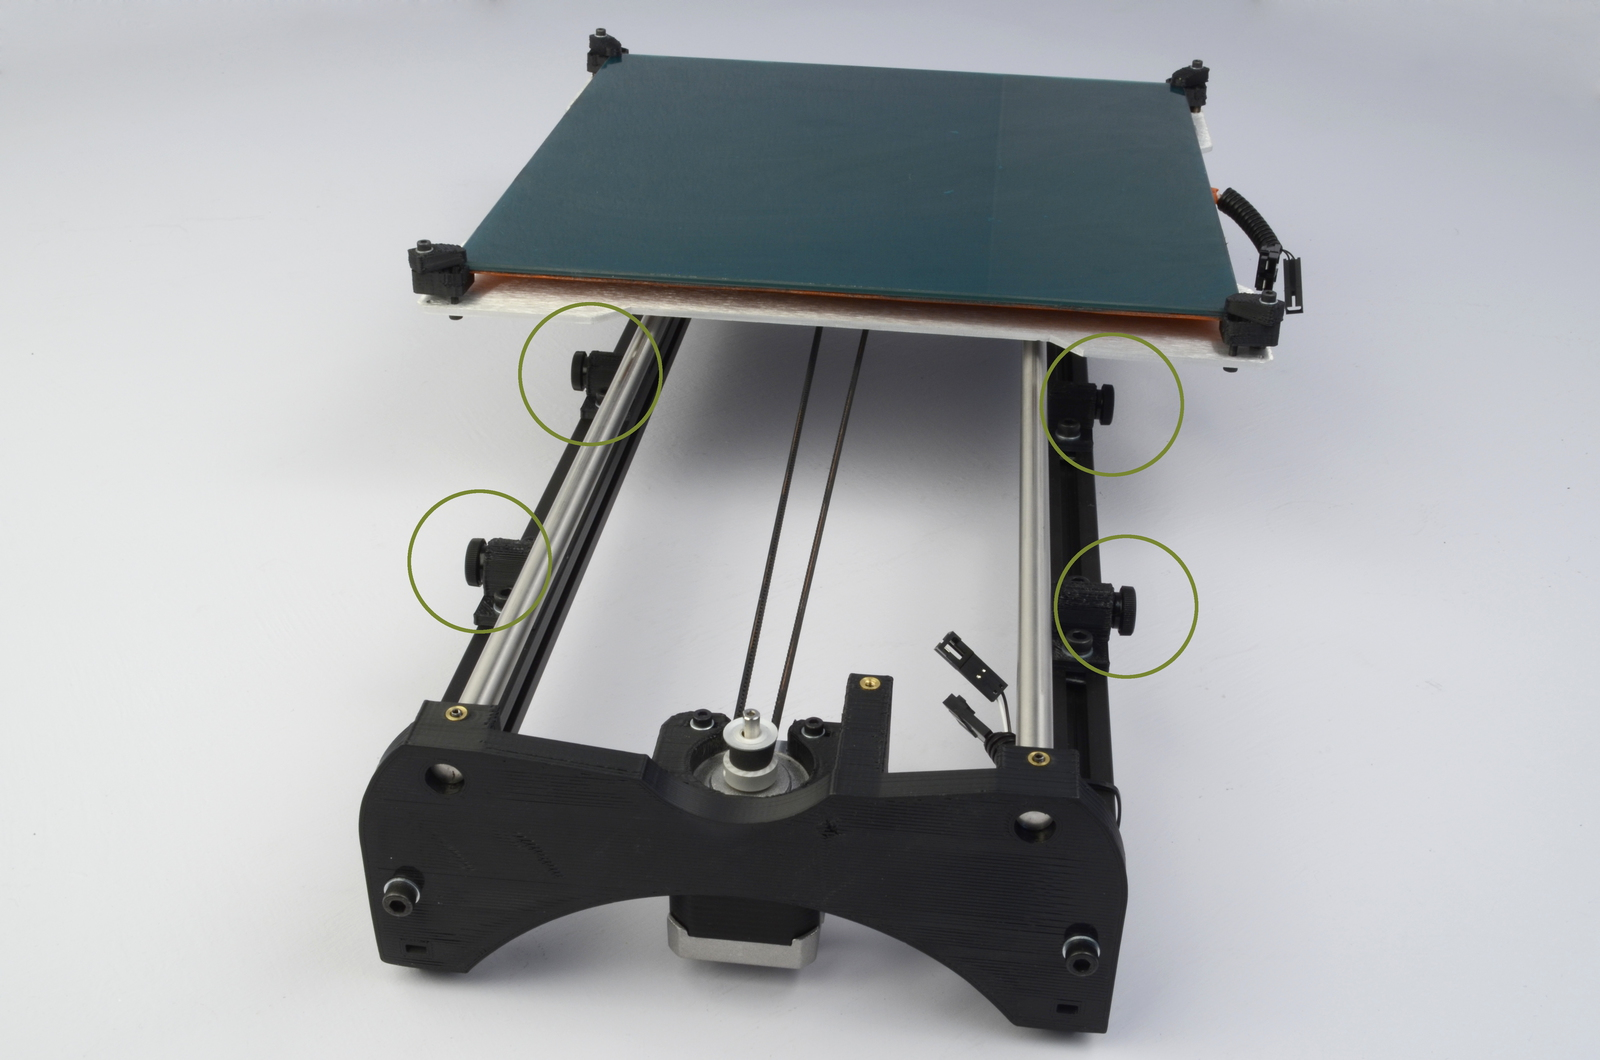
\includegraphics[keepaspectratio=true,angle=0,height=0.4\textheight,width=1.0\textwidth]{y_axis_bolts.JPG}
\caption{Locate the four Y axis bolts}
\label{fig:Y_axis_bolts}
\end{figure}

%\begin{figure}[hp] CD changed to force pic placement
\begin{figure}[H]
\centering
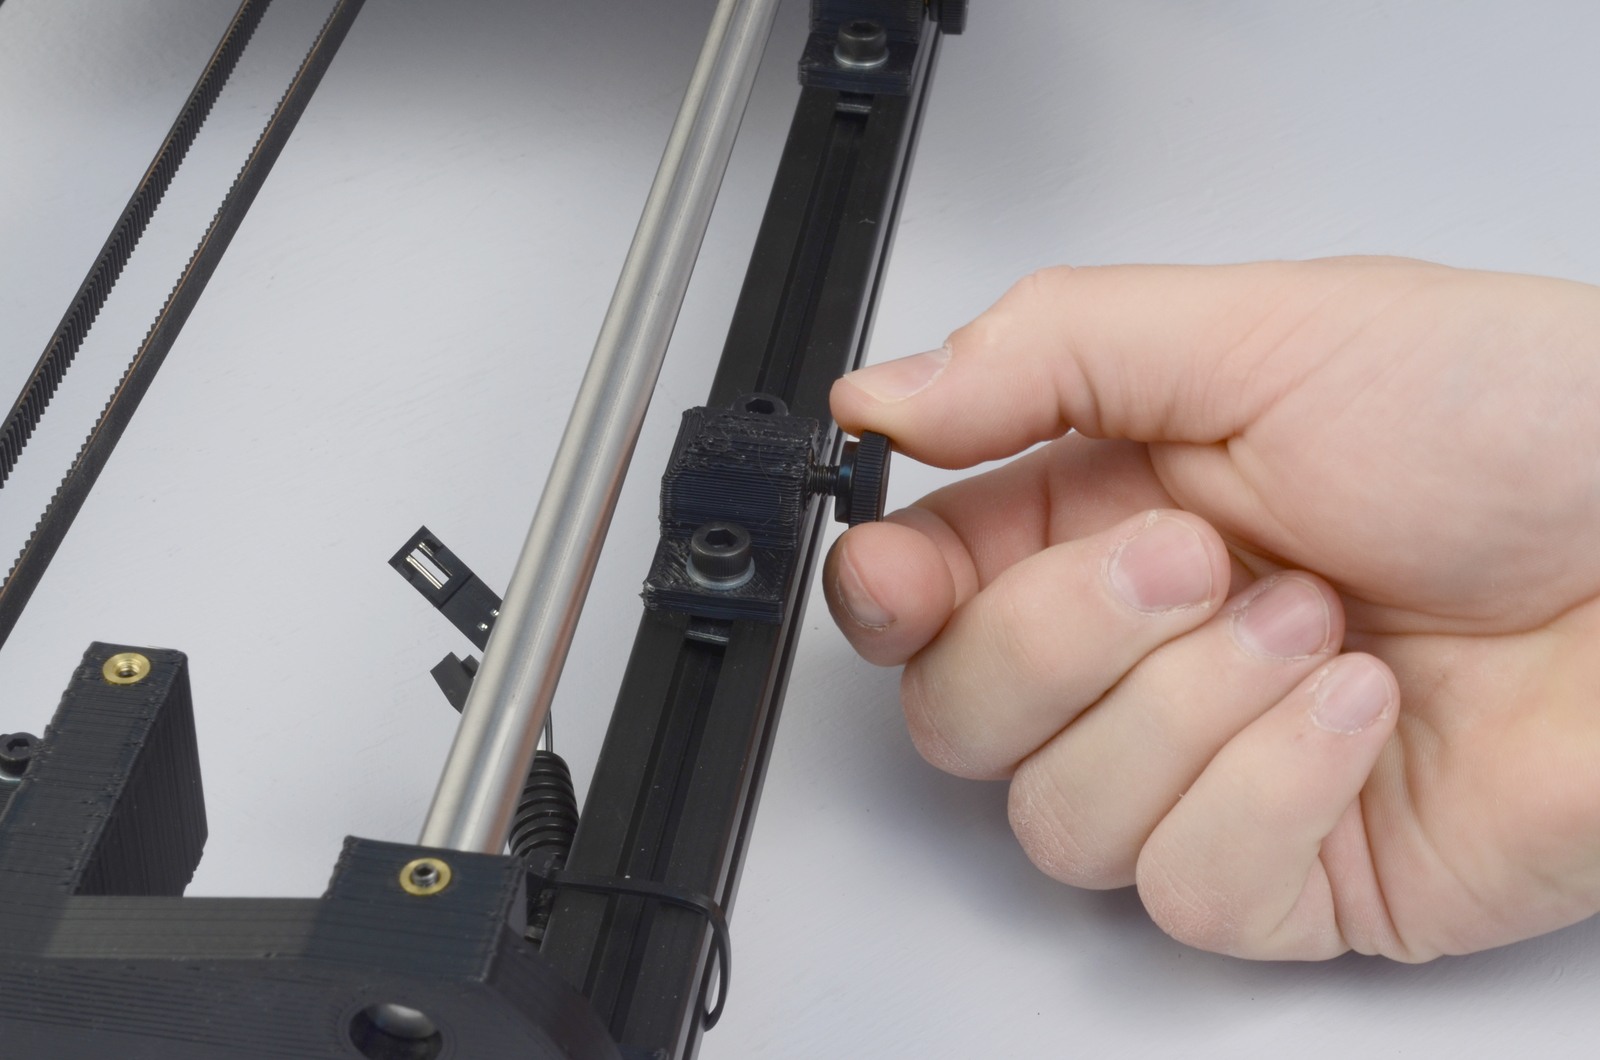
\includegraphics[keepaspectratio=true,angle=0,height=0.4\textheight,width=1.0\textwidth]{y_axis_bolt_remove.JPG}
\caption{Remove the four Y axis bolts}
\label{fig:remove_Y_axis_bolts}
\end{figure}

\item On the TAZ frame locate the four Y axis mount brackets shown in Fig. \ref{fig:frame_Y_axis_mounts} (pg. \pageref{fig:frame_Y_axis_mounts}). With the print surface facing up and the stepper motor end of the Y axis facing back, slide the Y axis assembly in between the Y axis mount brackets. The four Y axis mount brackets will line up with the Y axis bolt holes on the Y axis assembly. Thread the four Y axis bolts through the brackets, into the Y axis assembly (Fig. \ref{fig:Y_axis_bolts_tighten}, page \pageref{fig:Y_axis_bolts_tighten}). Before completely tightening the Y axis bolts make sure the Y axis aluminum bars are pushed down against the TAZ frame lower bars. You can do this by slightly tilting the printer, on the side edge, enough to lift the feet of the Y axis off of the table. The weight of the Y axis will seat it against the TAZ frame. While the printer is slightly tilted tighten the four Y axis bolts. The printer can now be set flat on the table.
%\begin{figure}[hp] CD forcing image placement
\begin{figure}[H]
\centering
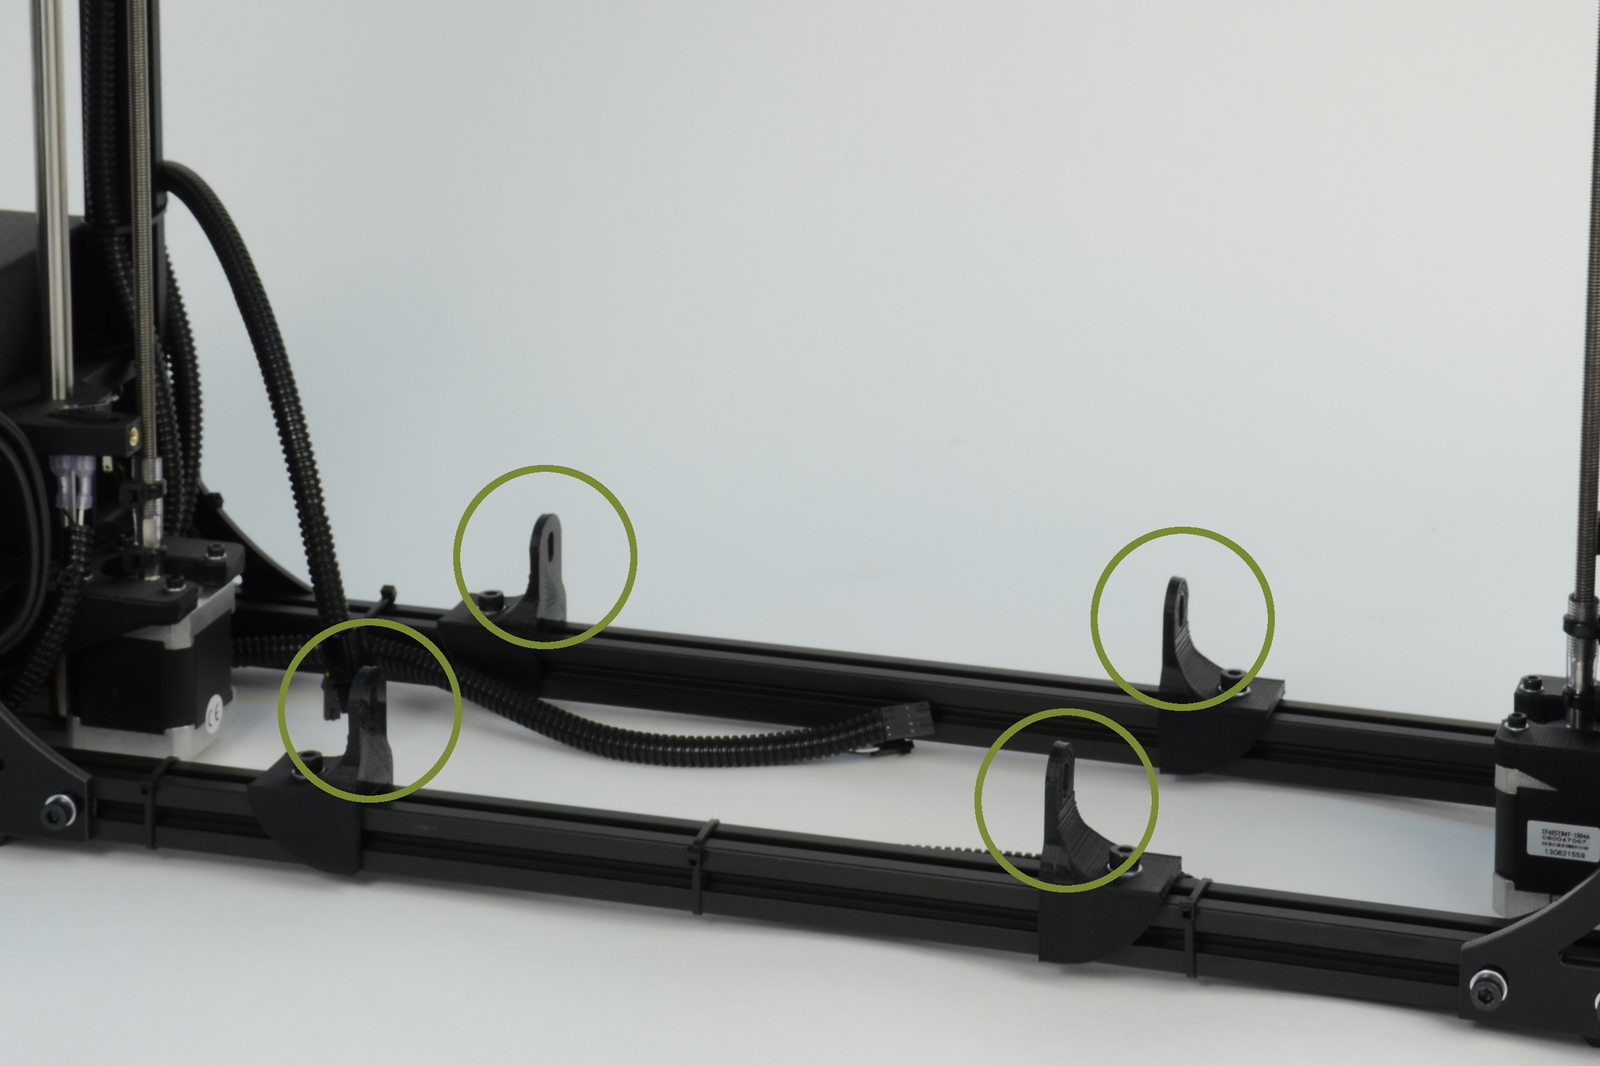
\includegraphics[keepaspectratio=true,angle=0,height=0.4\textheight,width=1.0\textwidth]{frame_y_axis_connector.JPG}
\caption{Locate the four Y axis mounts on the frame}
\label{fig:frame_Y_axis_mounts}
\end{figure}

%\begin{figure}[hp] CD forcing image placement
\begin{figure}[H]
\centering
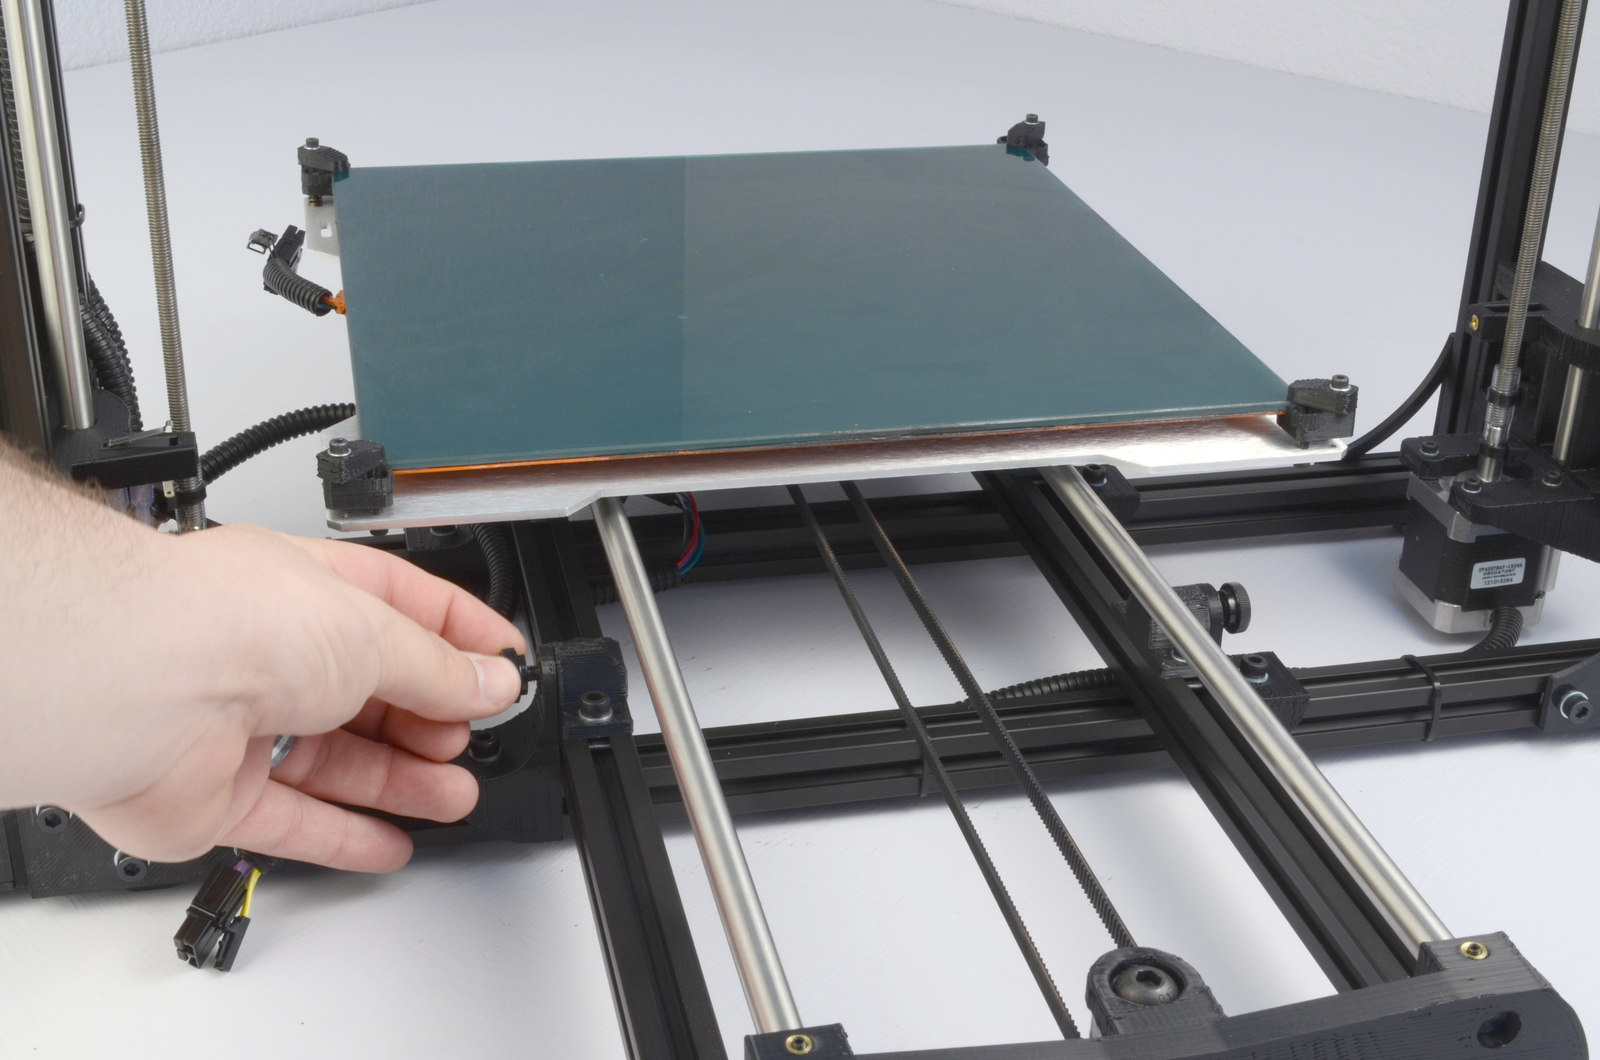
\includegraphics[keepaspectratio=true,angle=0,height=0.4\textheight,width=1.0\textwidth]{y_axis_bolt_tighten.JPG}
\caption{Screw in and tighten the four Y axis bolts}
\label{fig:Y_axis_bolts_tighten}
\end{figure}

\item The final step of installing the Y axis is connecting the print surface connectors and Y axis connectors. Pull the print bed completely to the front of the printer to get access to the Y axis connectors. You will find matching male and female 4 pin stepper motor connectors and two pin end stop connectors. Connect the matching male and female connectors (Fig. \ref{fig:Y_axis_connectors}, page \pageref{fig:Y_axis_connectors}); make sure the connector lock clicks to be sure that the connection is secure.


\begin{figure}[H]
\centering
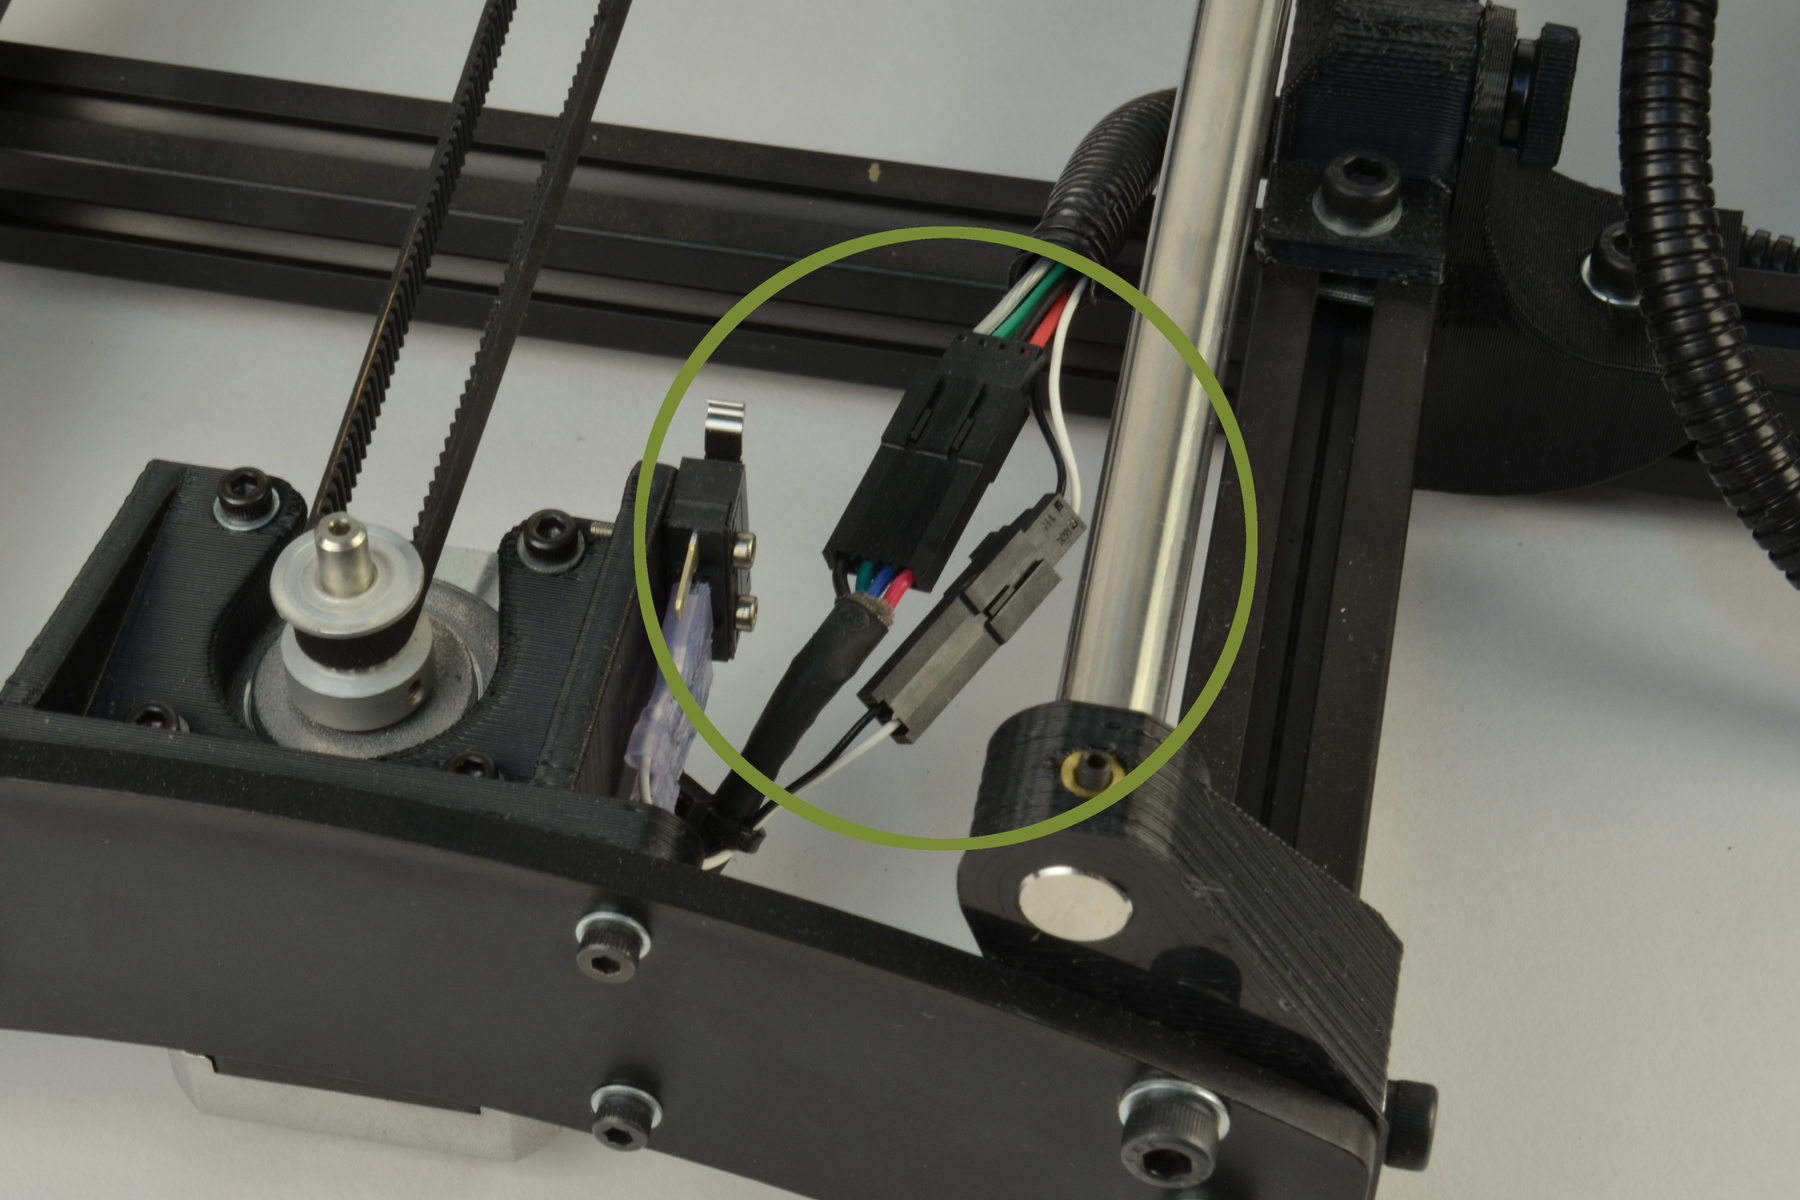
\includegraphics[keepaspectratio=true,angle=0,height=0.4\textheight,width=1.0\textwidth]{y_axis_connectors.JPG}
\caption{Connect the two connectors found at the rear of the Y axis}
\label{fig:Y_axis_connectors}
\end{figure}

\item Locate the two connectors to the left of the print bed. Connect the matching female and male large two pin heat bed connectors and the small two pin thermistor connectors, again making sure the connectors lock(Fig. \ref{fig:bed_connectors}, page \pageref{fig:bed_connectors}).

\begin{figure}[H]
\centering
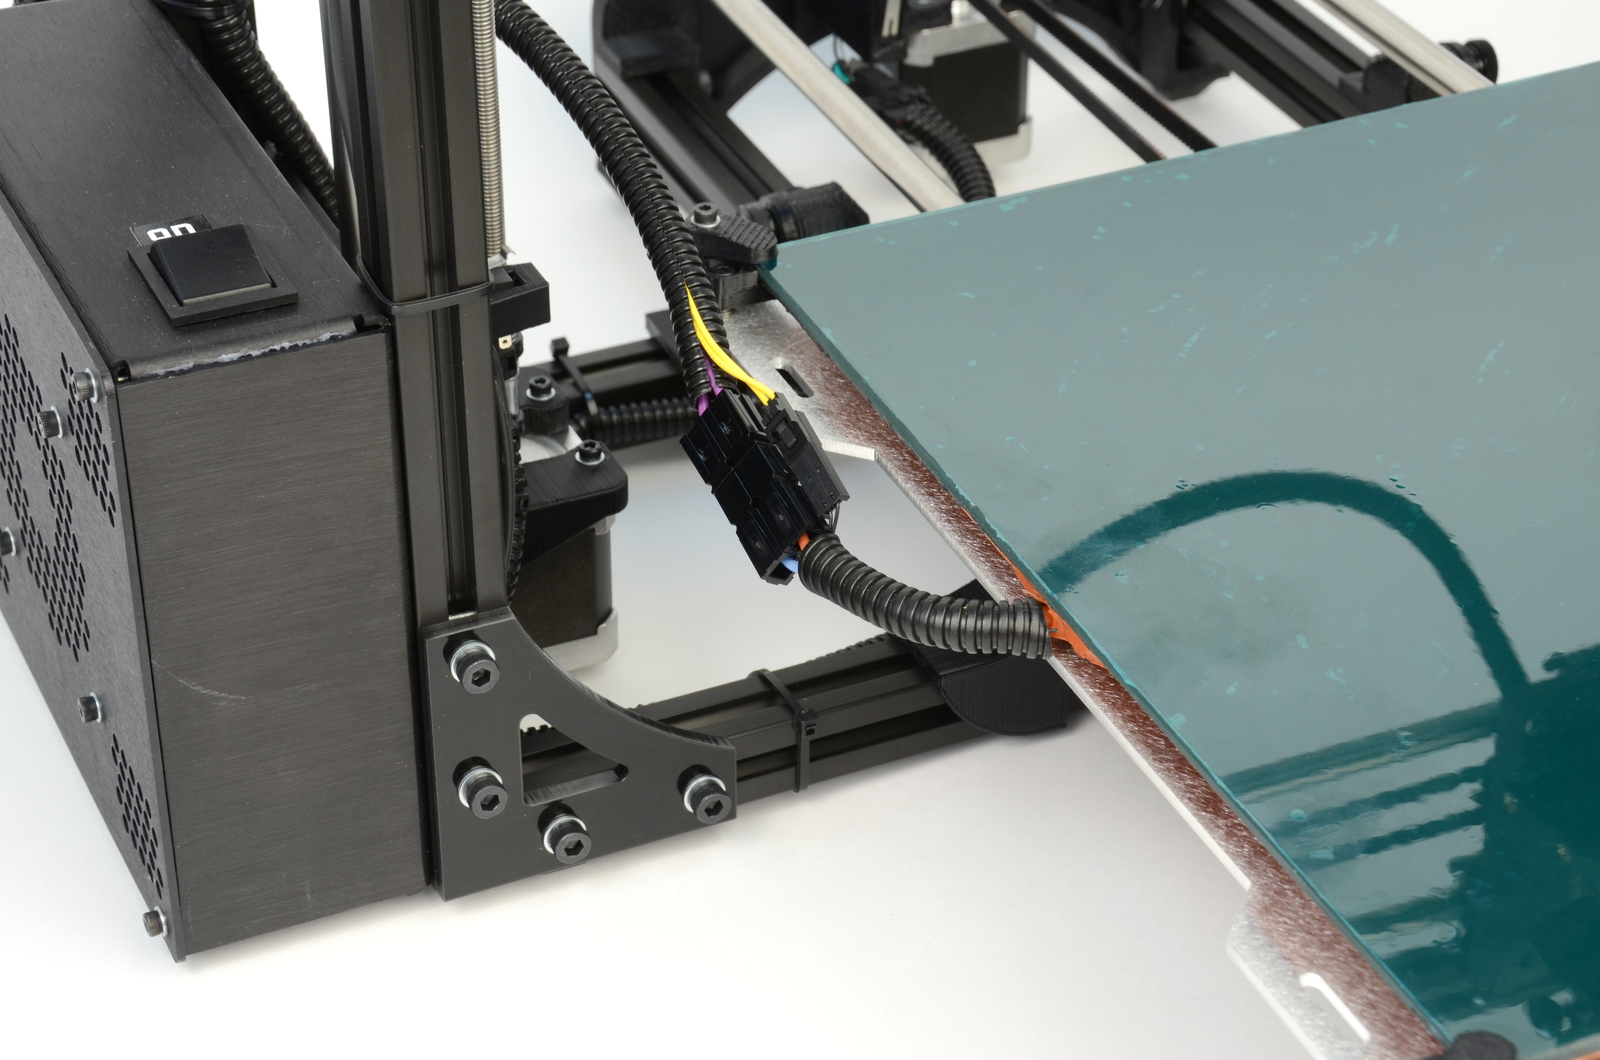
\includegraphics[keepaspectratio=true,angle=0,height=0.4\textheight,width=1.0\textwidth]{bed_connectors.JPG}
\caption{Connect the two connectors on the left of the print bed}
\label{fig:bed_connectors}
\end{figure}

\item Locate the two small black zip ties that are included in the documents bag (Fig. \ref{fig:bed_connectors_strain_relief}, page \pageref{fig:bed_connectors_strain_relief}). Wrap the two zip ties through the slot, located on the left rear of the aluminum bed plate, and around the print bed wires (Fig. \ref{fig:bed_connectors_strain_relief_done}, page \pageref{fig:bed_connectors_strain_relief_done}). Tighten the zip ties snug so the wire cannot move freely. Cut off the excess end of the zip ties with the needle nose pliers included in the tool bag.

%\begin{figure}[hp] CD forcing image placement
\begin{figure}[H]
\centering
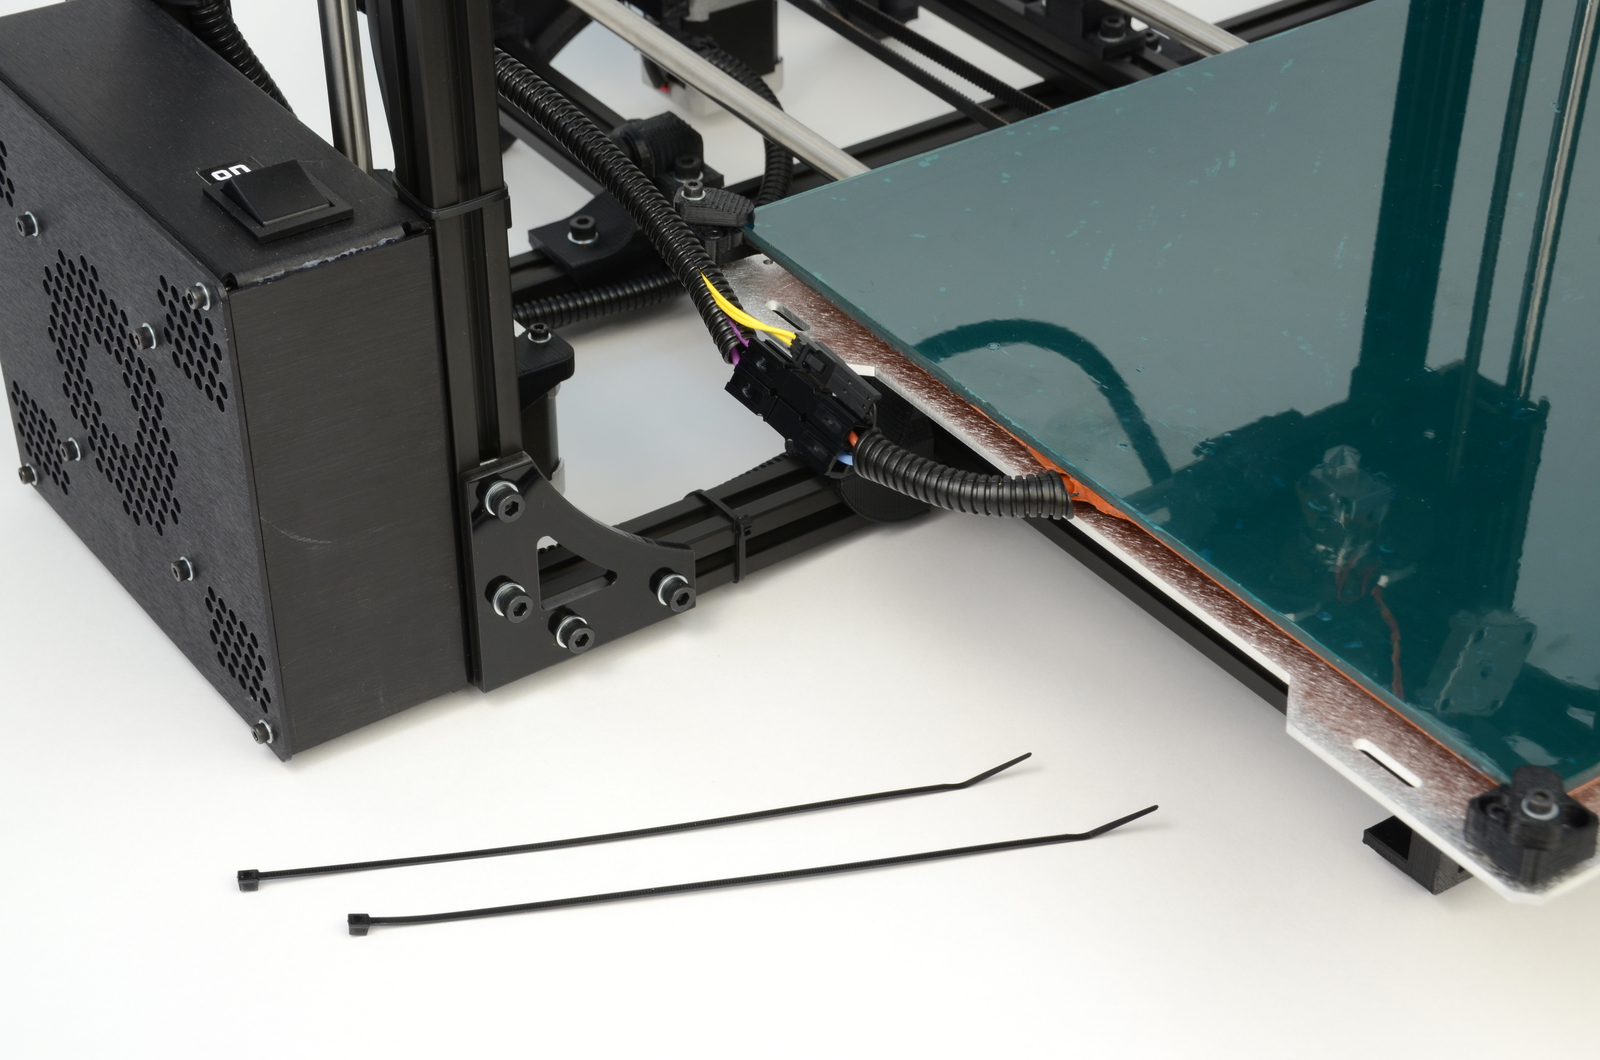
\includegraphics[keepaspectratio=true,angle=0,height=0.4\textheight,width=1.0\textwidth]{bed_connectors_strain_relief.JPG}
\caption{Locate the two zip ties found in the bag with the manual}
\label{fig:bed_connectors_strain_relief}
\end{figure}

%\begin{figure}[hp] CD forcing image placement
\begin{figure}[H]
\centering
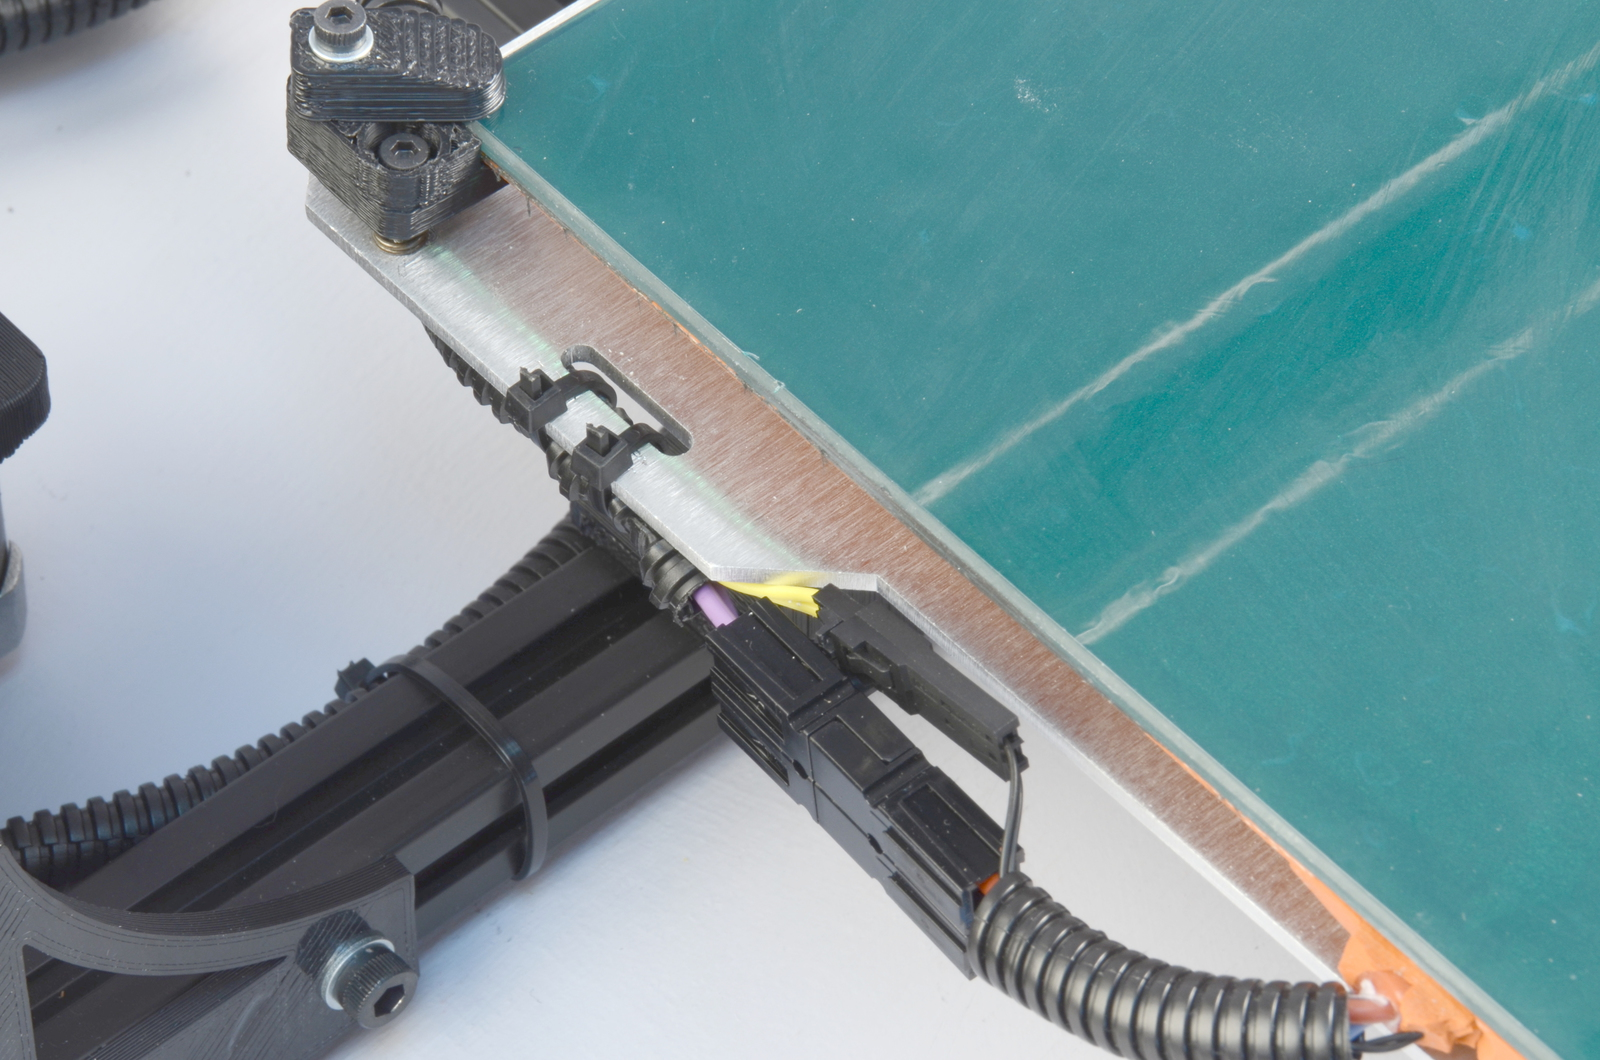
\includegraphics[keepaspectratio=true,angle=0,height=0.4\textheight,width=1.0\textwidth]{bed_connectors_strain_relief_done.JPG}
\caption{Tightly wrap the zip ties around the bed wires and through the strain relief slot}
\label{fig:bed_connectors_strain_relief_done}
\end{figure}

\item Move the X axis carriage to the center of the smooth rods. If you have not already done so, remove the foam from between the X axis carriage and the left hand X axis end. Locate and remove, with the 2.5mm hex driver, the tool head 3mm screw in top center of the X axis carriage (Fig. \ref{fig:tool_head_screw}, page \pageref{fig:tool_head_screw}). Place the extruder tool head mount onto the X axis carriage bottom first. The extruder mount will slide into the bottom portion of the carriage and self center (Fig. \ref{fig:tool_head_placement}, page \pageref{fig:tool_head_placement}). Use the included 2.5mm driver and the previously removed 3mm screw to secure the extruder tool head onto the X axis carriage.
\begin{figure}[hp]
\centering
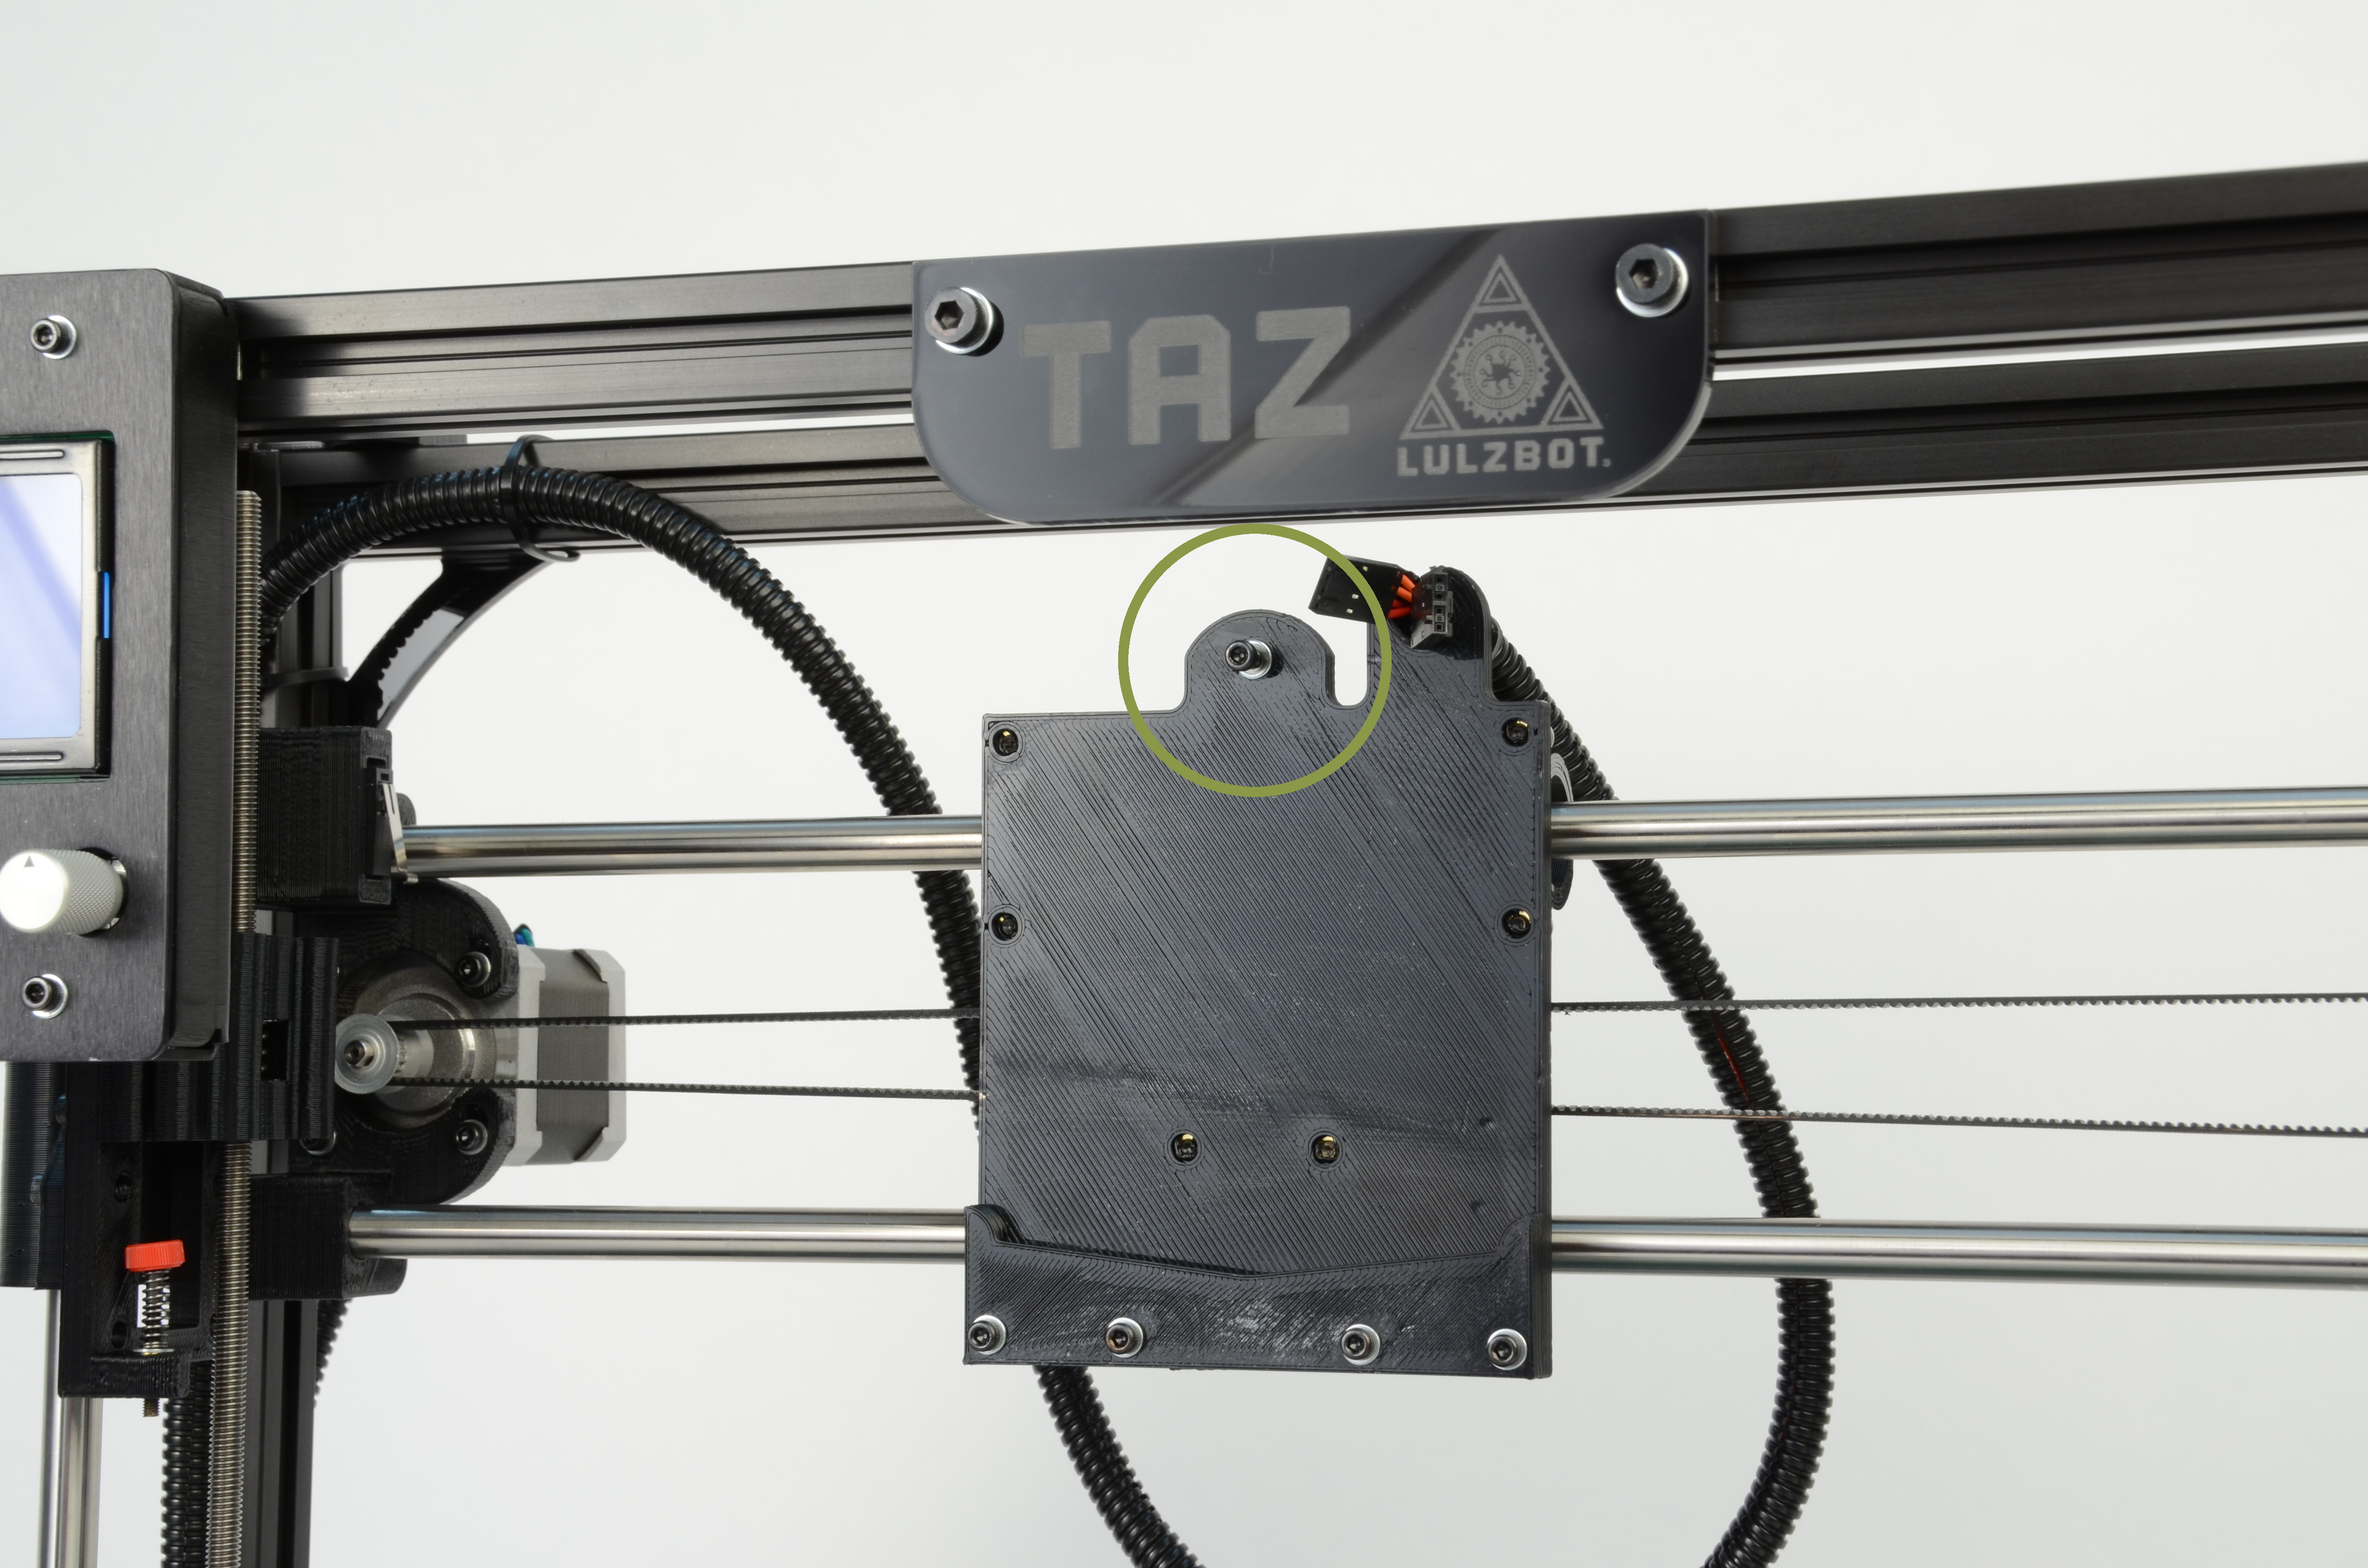
\includegraphics[keepaspectratio=true,angle=0,height=0.4\textheight,width=1.0\textwidth]{tool_head_screw.JPG}
\caption{Remove the tool head screw}
\label{fig:tool_head_screw}
\end{figure}

\begin{figure}[hp]
\centering
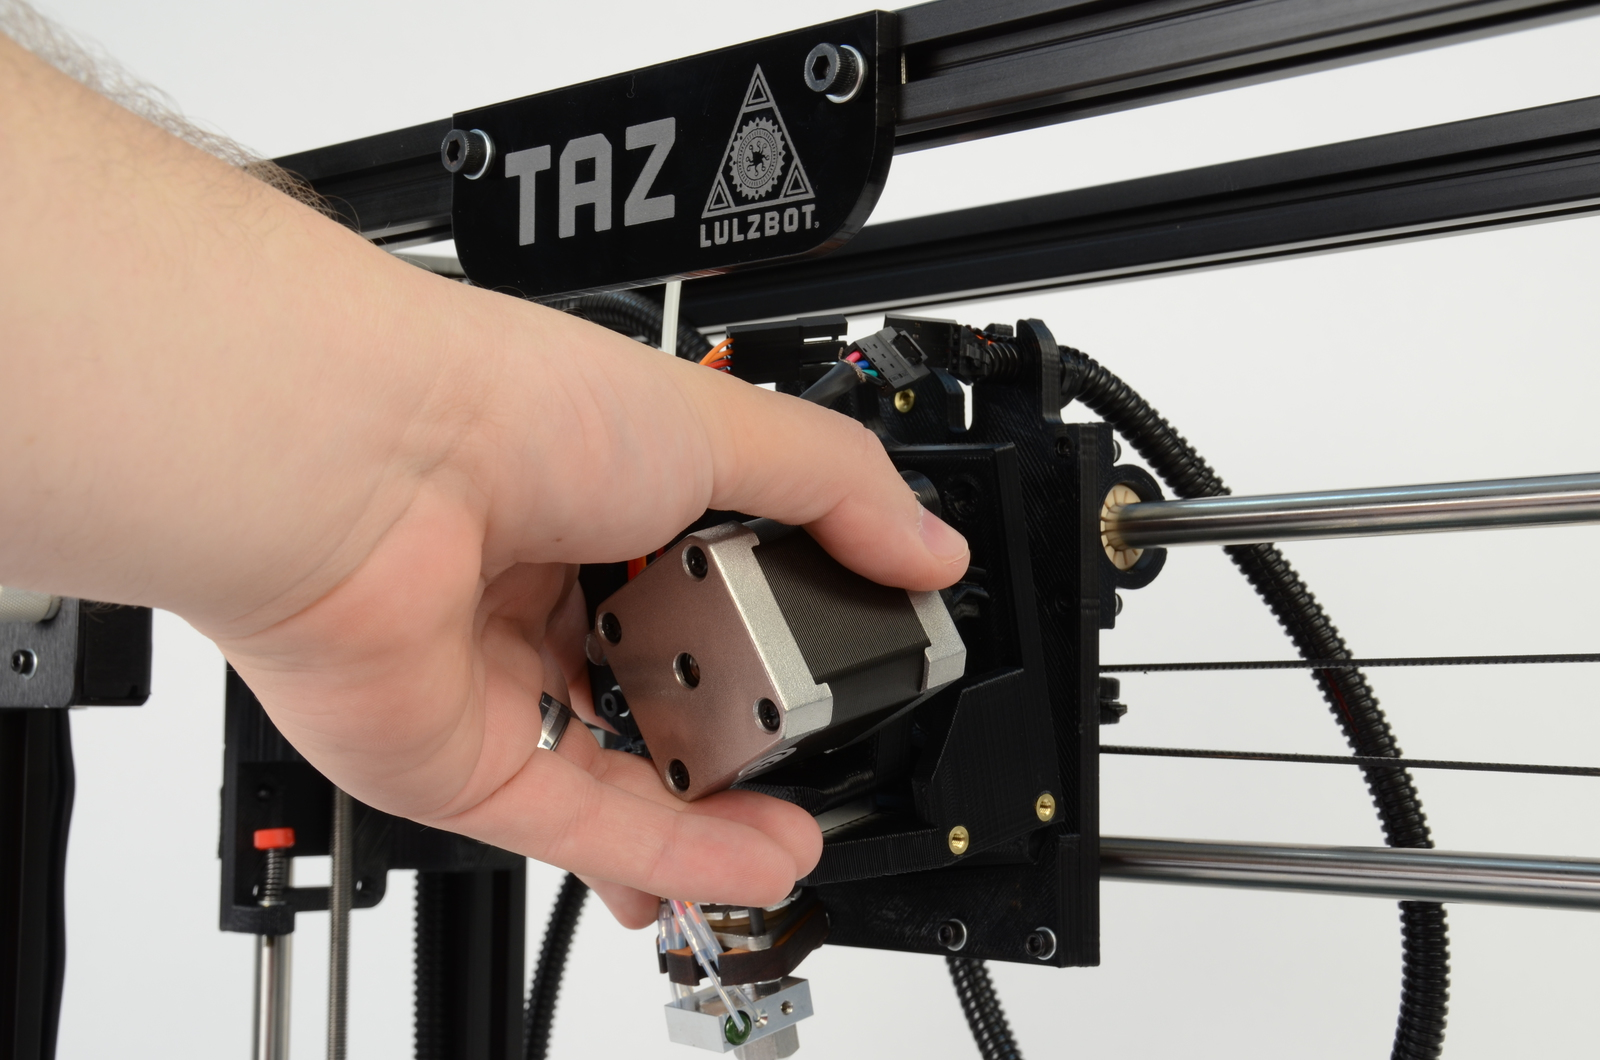
\includegraphics[keepaspectratio=true,angle=0,height=0.4\textheight,width=1.0\textwidth]{tool_head_placement.JPG}
\caption{Mount the extruder tool head}
\label{fig:tool_head_placement}
\end{figure}

\begin{figure}[hp]
\centering
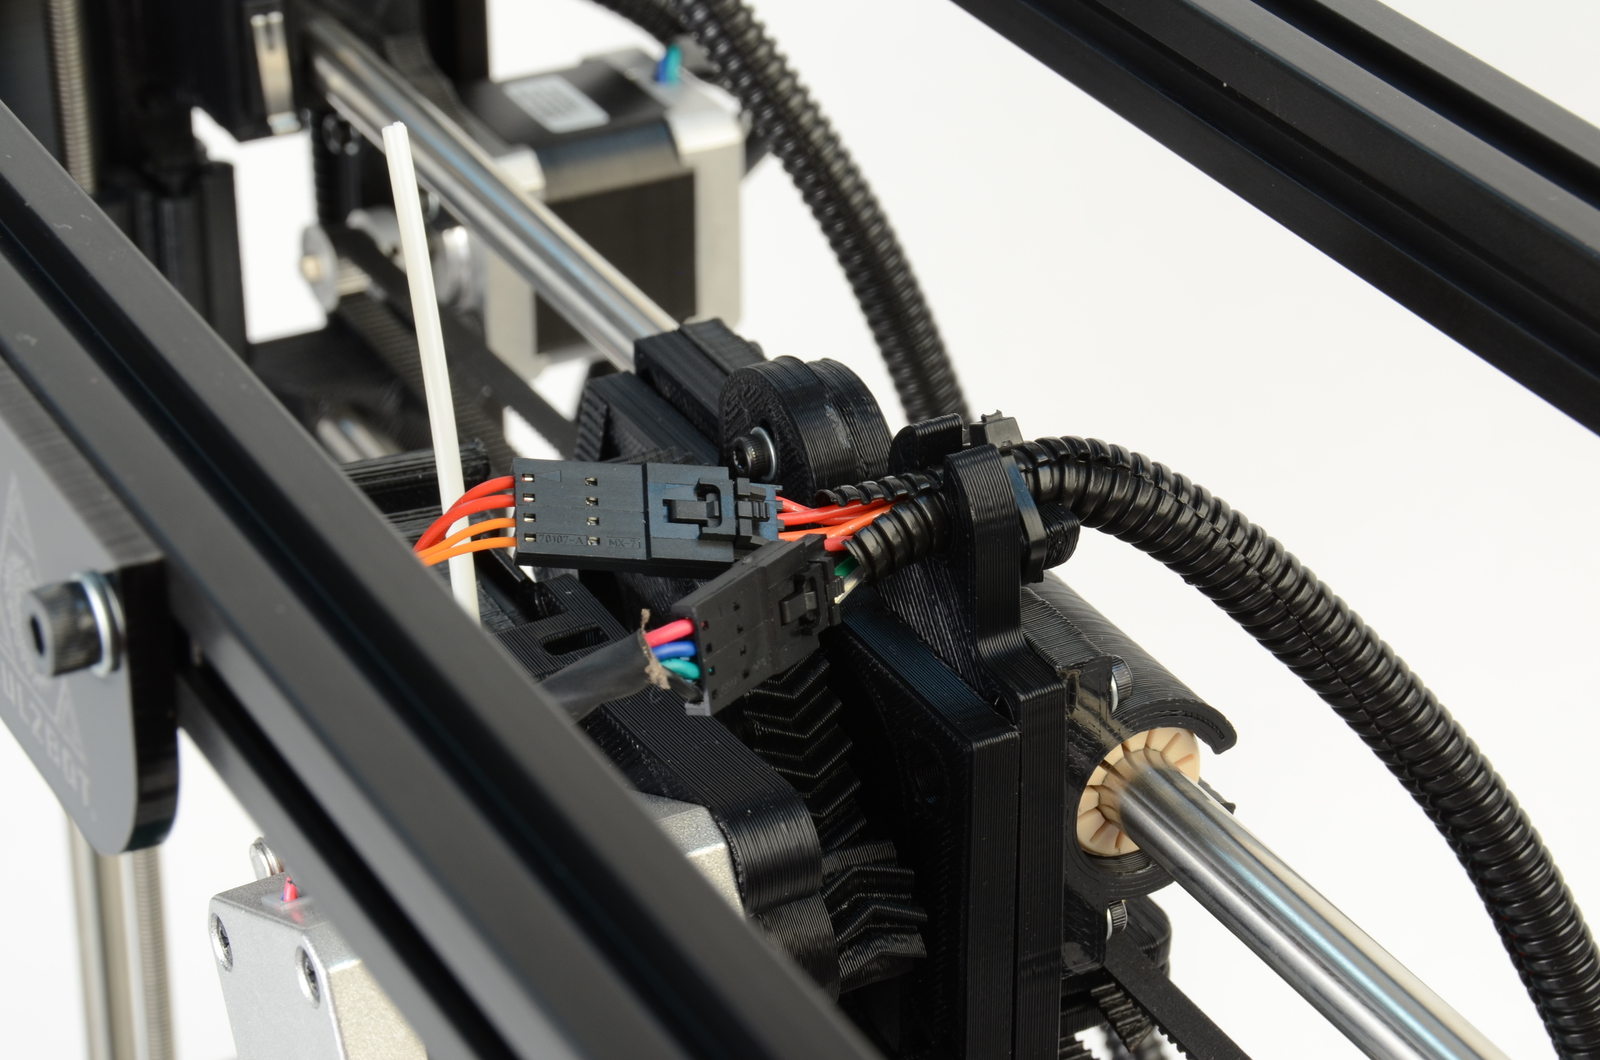
\includegraphics[keepaspectratio=true,angle=0,height=0.4\textheight,width=1.0\textwidth]{tool_head_connectors.JPG}
\caption{Connect the two tool head connectors}
\label{fig:tool_head_connectors}
\end{figure}

\item Connect the stepper motor and the hot end to the existing wiring harness located at the top of the X axis carriage. You will find matching colored male and female 4 pin connectors. Connect the matching male and female connectors for the extruder stepper motor and hot end (Fig. \ref{fig:tool_head_connectors}, page \pageref{fig:tool_head_connectors}); orange/yellow wired connecters paired and red/blue/green/black wired connectors paired. Make sure the connector locks click to be sure that the connections are secure.

\item Now that the Y axis is mounted and the extruder tool head is installed you should set your printer on a stable, flat, and level surface large enough for extra space around the printer. Make sure your printer work space is clear of anything that could obstruct the movement of the printer. Move the Y axis to the back of the printer to ensure unobstructed movement of that axis. \textcolor{red}{Make sure there are no flammable fabrics or liquids near the printer space}. It is also best to not put your printer near a drafty window or air conditioner vent.

\index{power supply}
\index{USB cable}
\item Unwrap the power supply and USB cables.

\textcolor{red}{MAKE SURE THE POWER SUPPLY IS COMPLETELY UNPLUGGED BEFORE MOVING ON TO THE NEXT STEP}.

\index{electronics receptacles}
\item Locate the power supply and USB receptacles along the back of the TAZ electronics enclosure
(Fig. \ref{fig:electronics_plugs}, page \pageref{fig:electronics_plugs}). Locate the power supply and the included AC power cable (Fig. \ref{fig:power_supply}, page \pageref{fig:power_supply}). Locate the DC power cable plug on the power supply. Connect the DC locking plug into the DC connector on the TAZ electronics enclosure (Fig. \ref{fig:ps_plug}, page \pageref{fig:ps_plug}). The plug is keyed which may require rotating the plug until the keys line up and the plug can be pushed in. Once you have pushed in the plug turn the locking sleeve clockwise until it is tight against the electronics enclosure (Fig. \ref{fig:electronics_plugs_plugged-in}, page \pageref{fig:electronics_plugs_plugged-in}).
%\begin{figure}[hbt]
\begin{figure}[H]
\centering
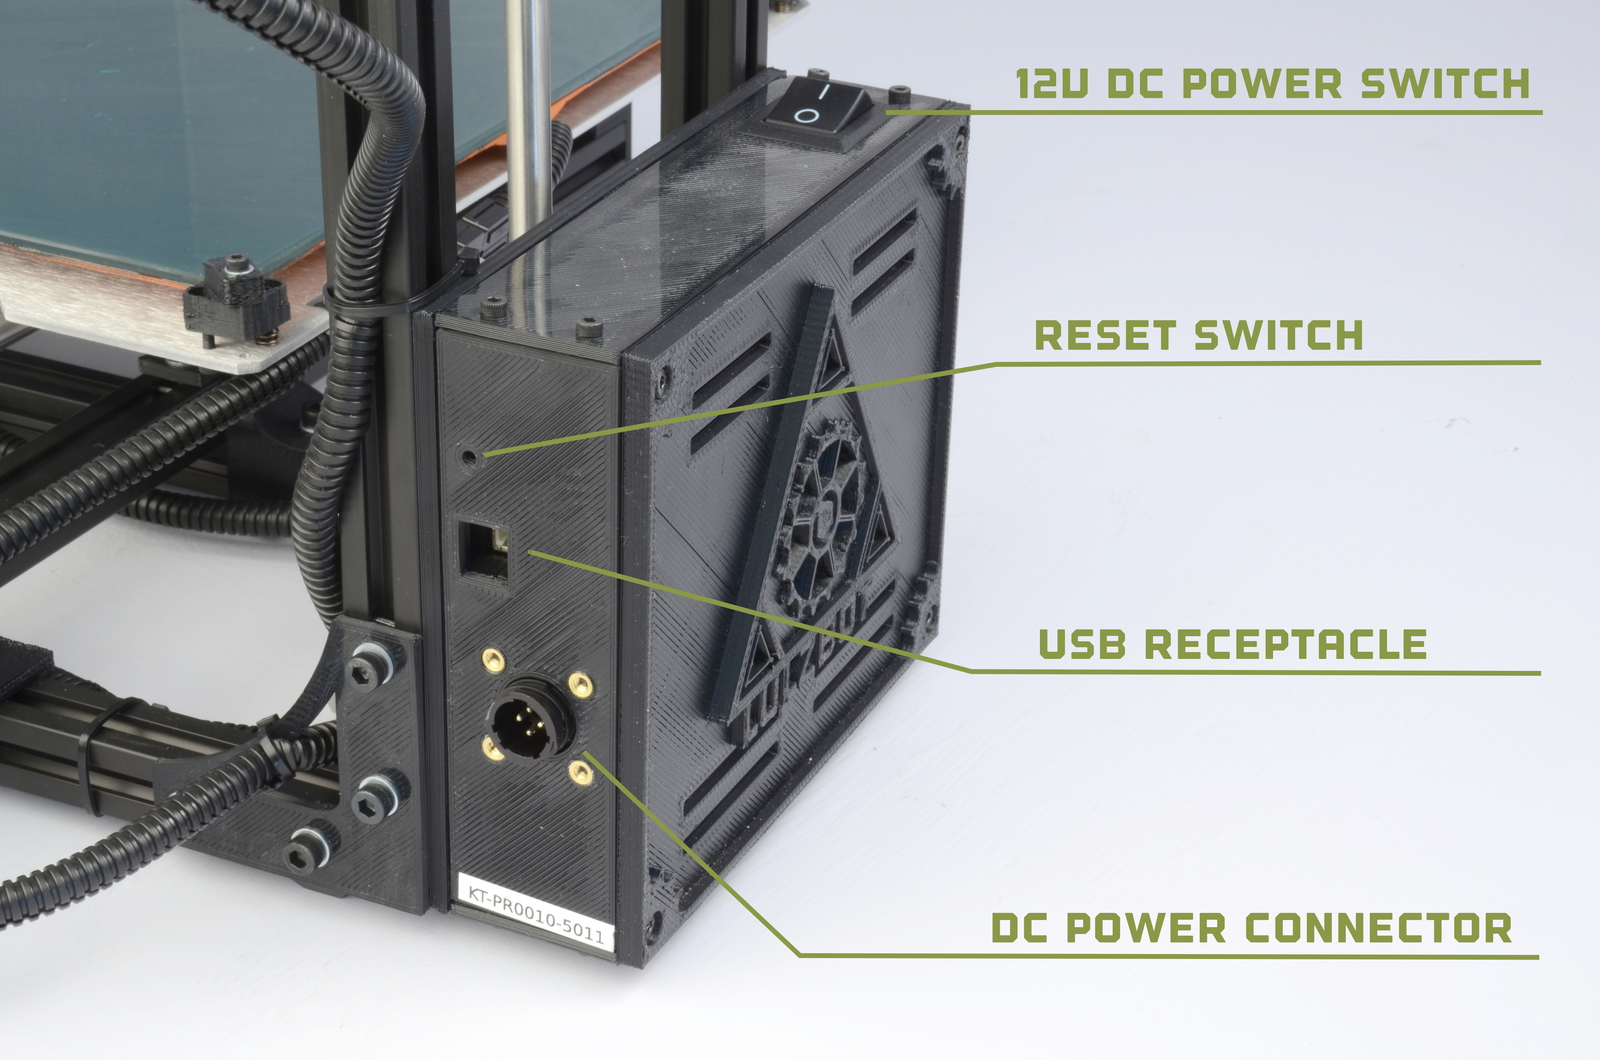
\includegraphics[keepaspectratio=true,angle=0,height=0.4\textheight,width=1.0\textwidth]{electronics_case_rec.JPG}
\caption{Power supply and USB receptacles}
\label{fig:electronics_plugs}
\end{figure}

%\begin{figure}[hp]
\begin{figure}[H]
\centering
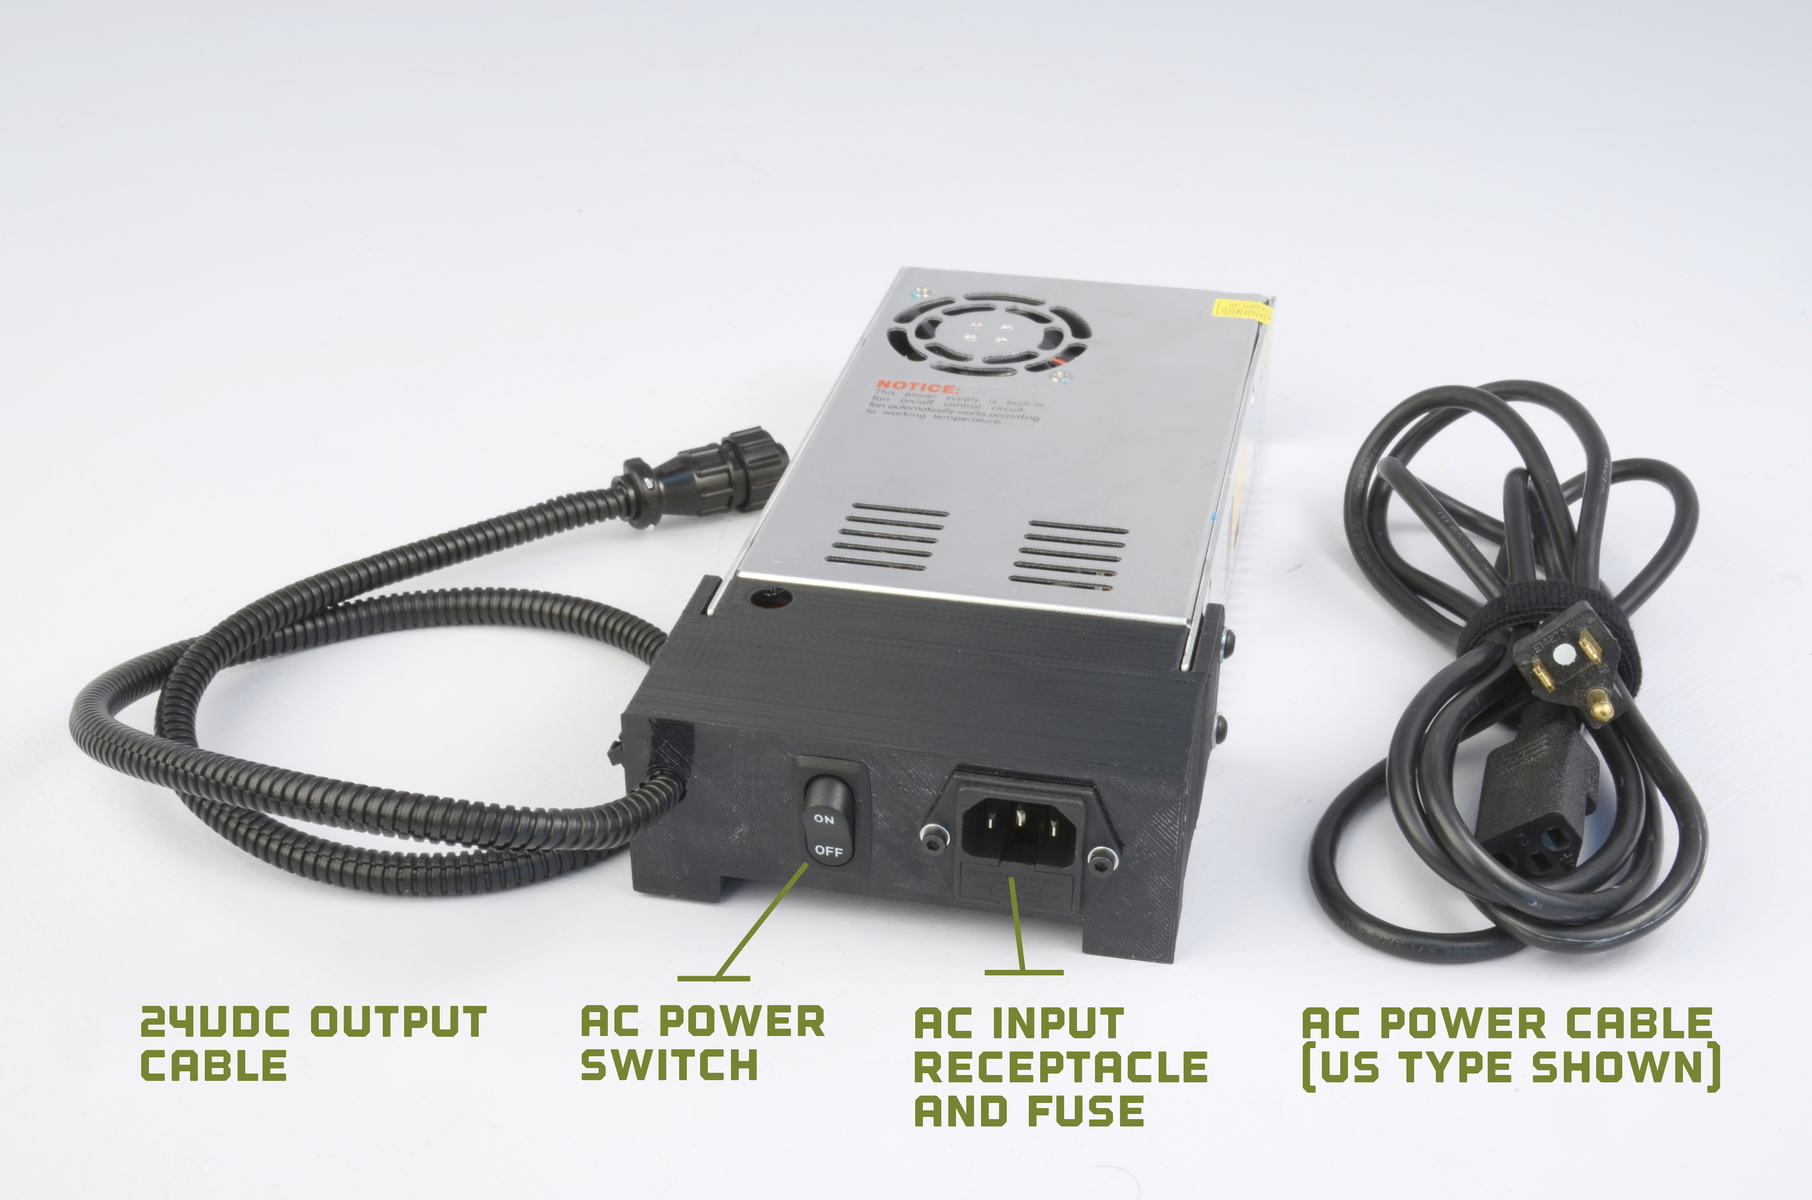
\includegraphics[keepaspectratio=true,angle=0,height=0.4\textheight,width=1.0\textwidth]{power_supply.JPG}
\caption{Power supply}
\label{fig:power_supply}
\end{figure}

%\begin{figure}[hp]
\begin{figure}[H]
\centering
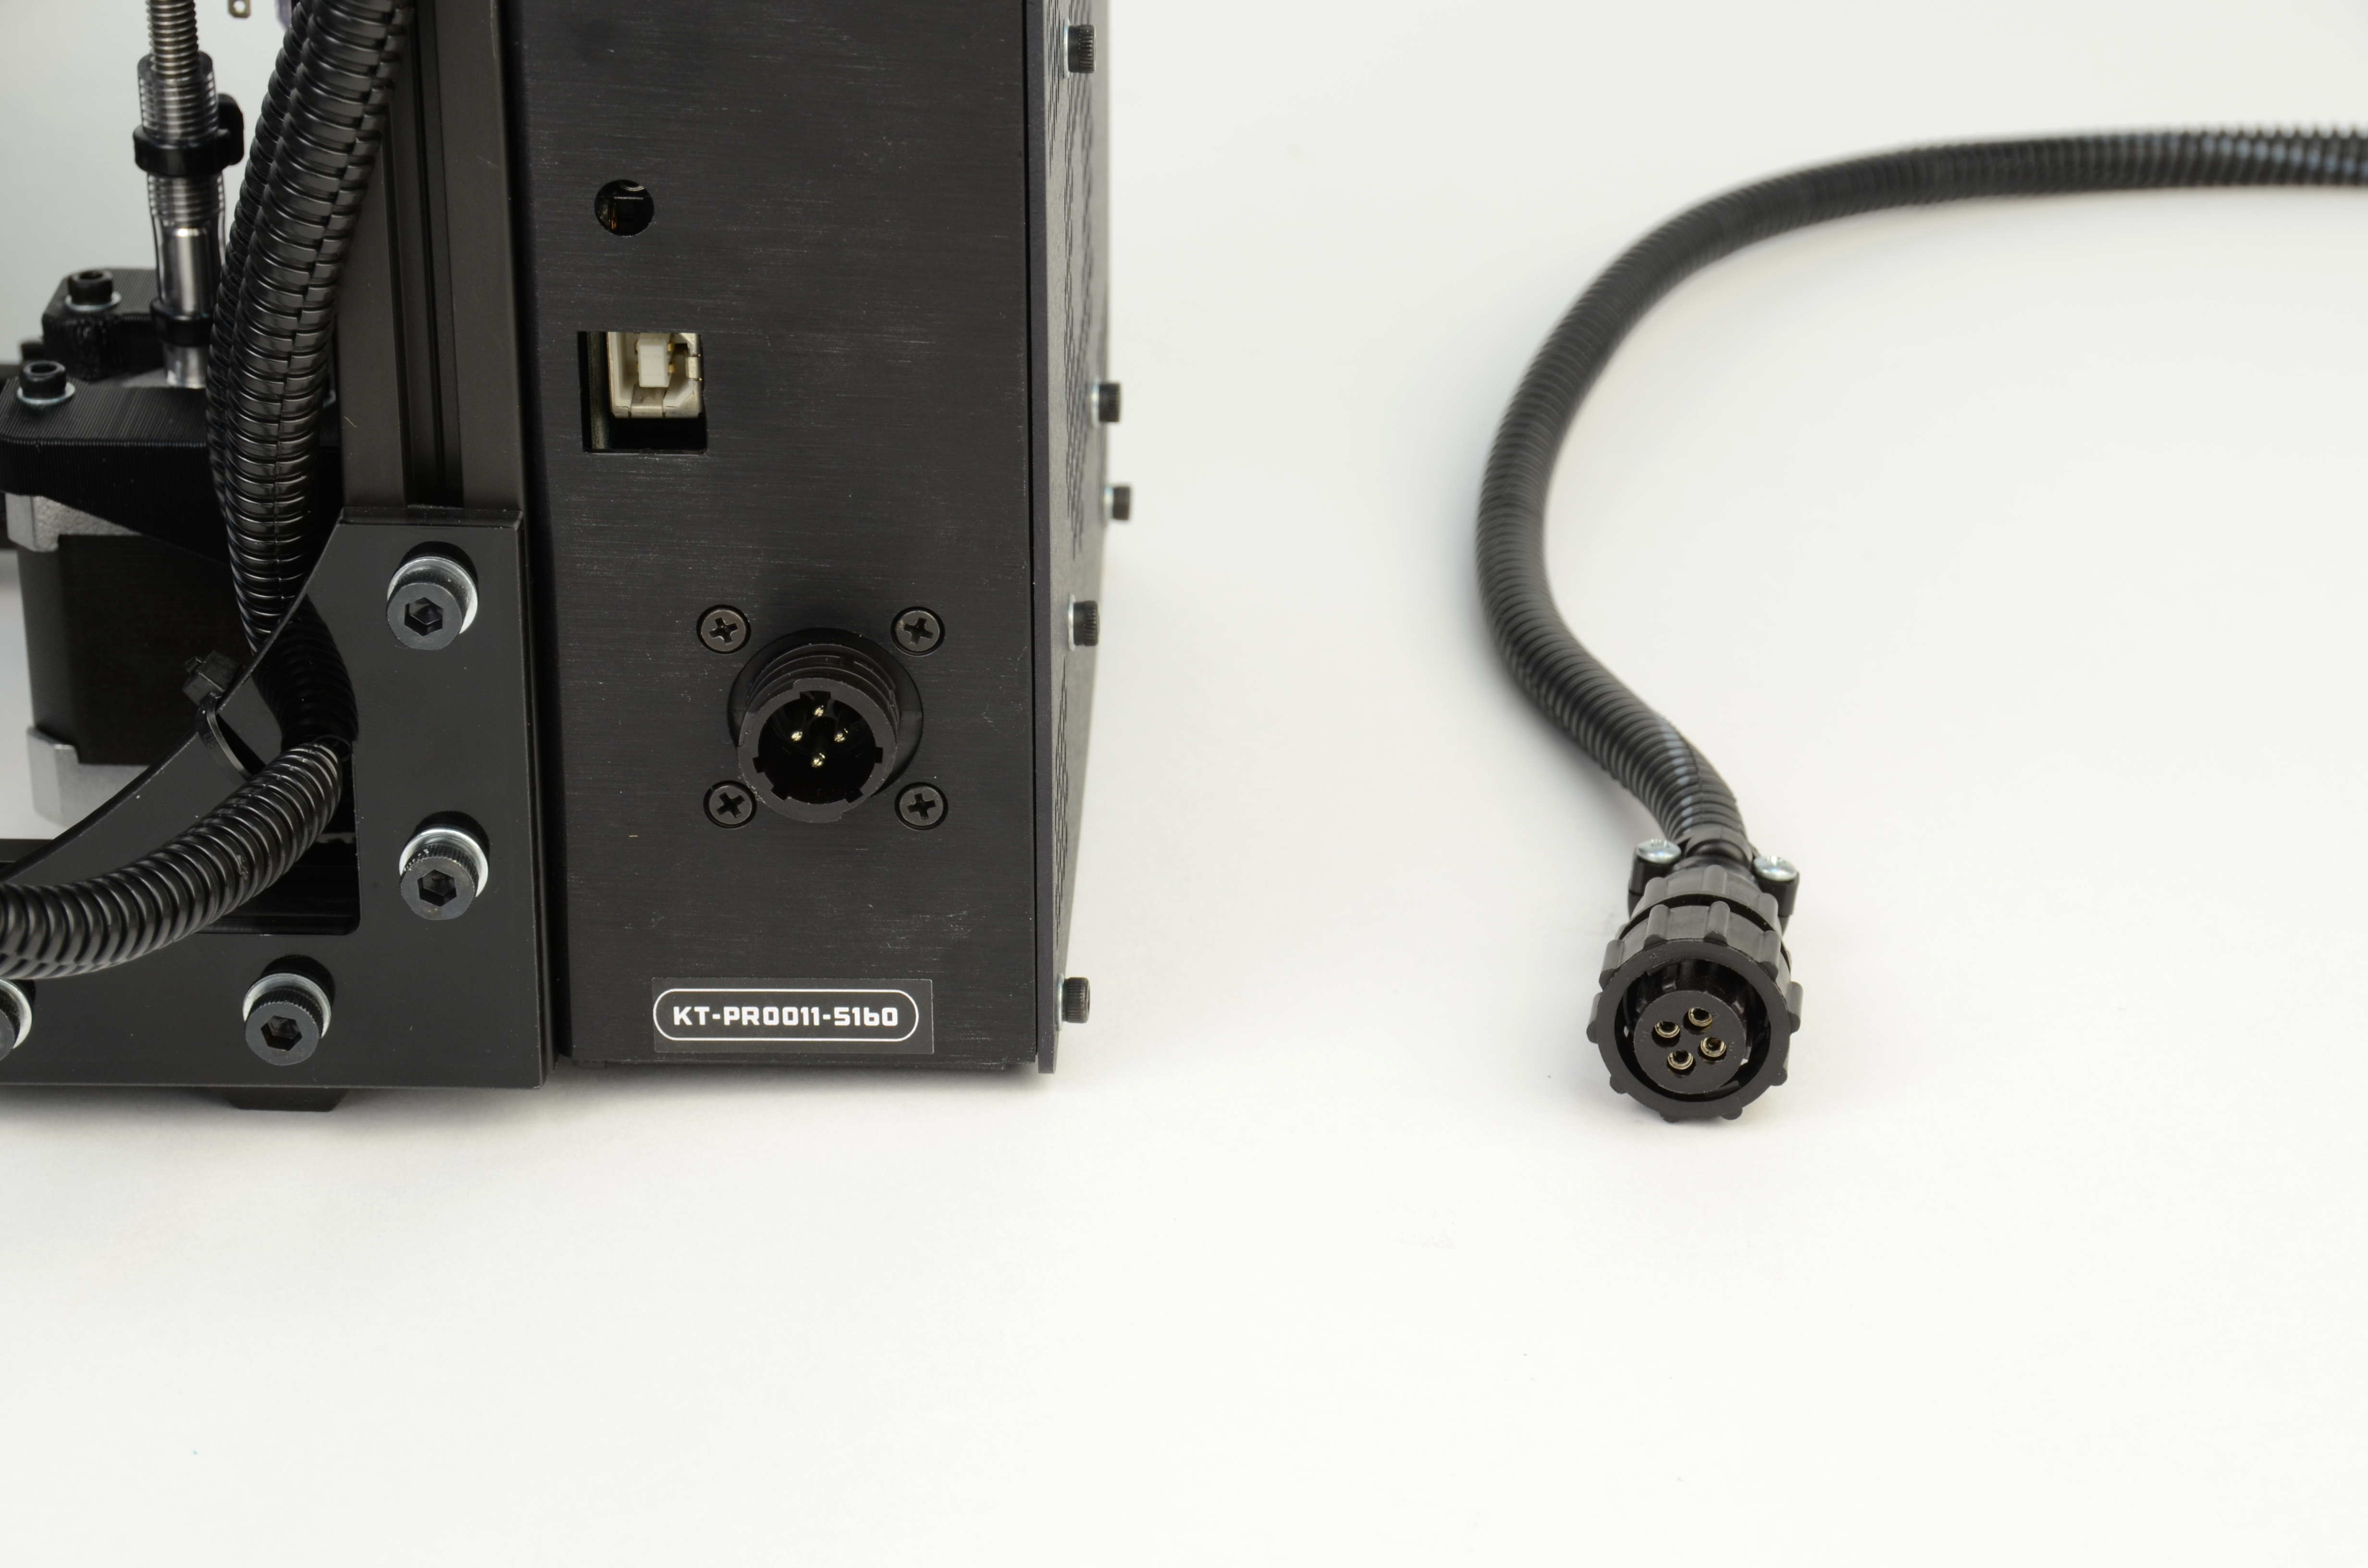
\includegraphics[keepaspectratio=true,angle=0,height=0.4\textheight,width=1.0\textwidth]{electronics_DC_connector.JPG}
\caption{12V DC Power supply plug and receptacle}
\label{fig:ps_plug}
\end{figure}

%\begin{figure}[hp]
\begin{figure}[H]
\centering
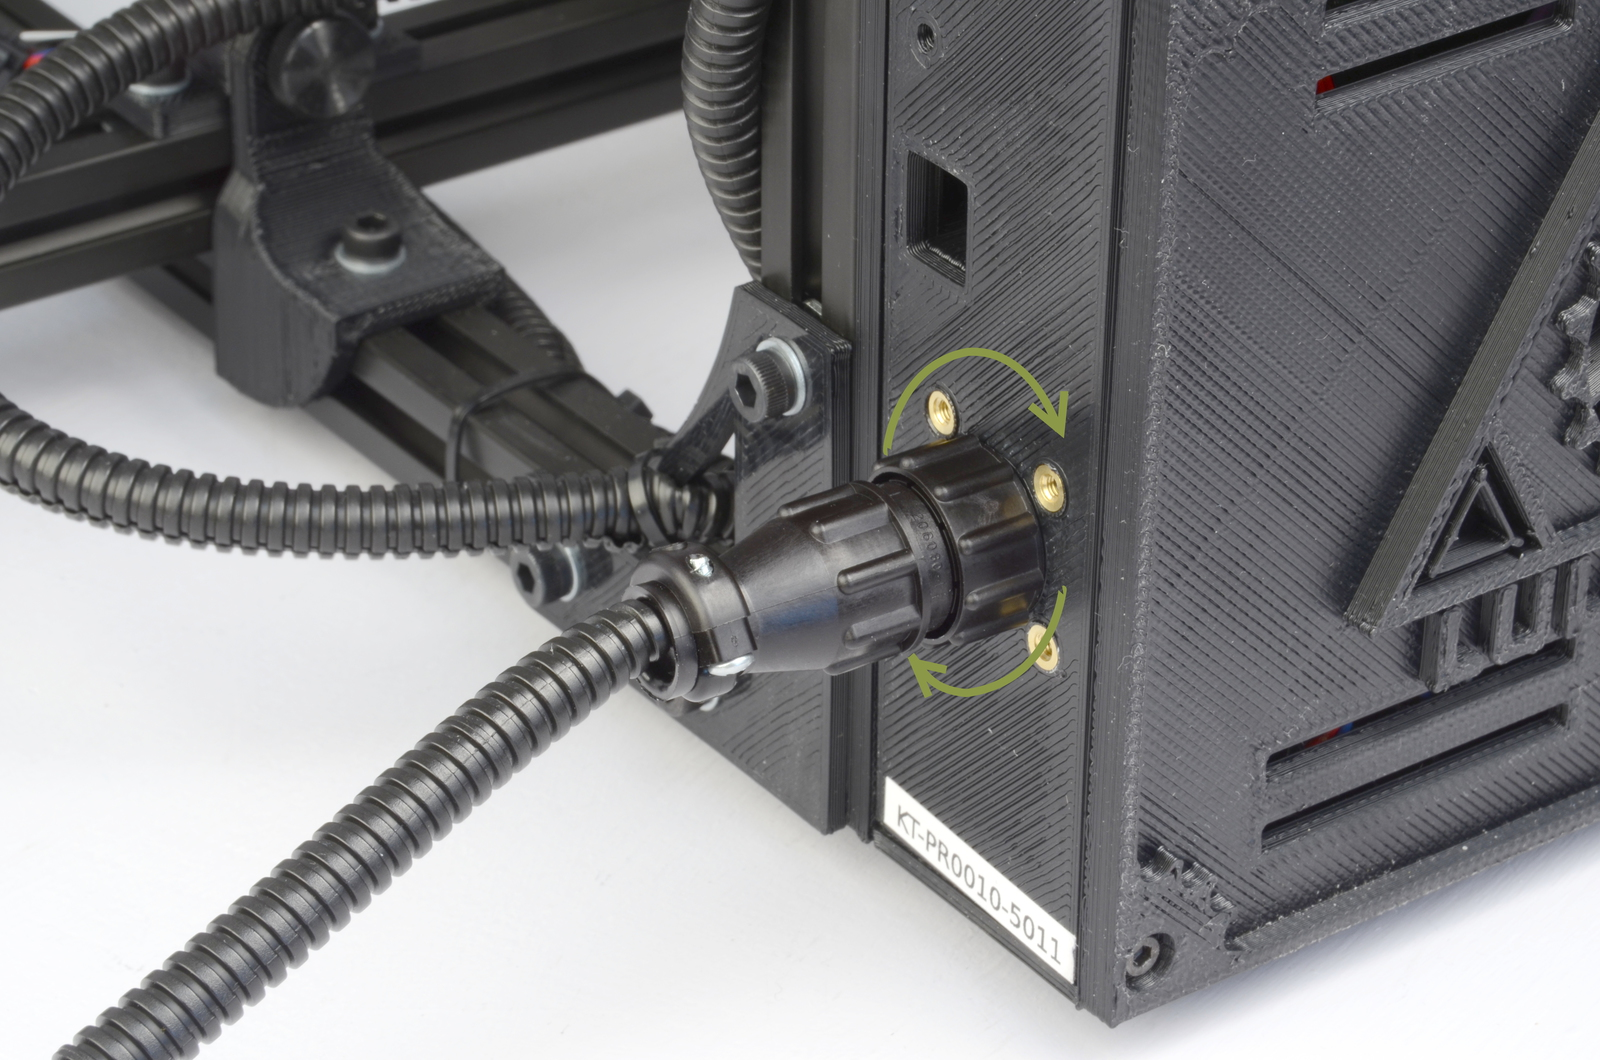
\includegraphics[keepaspectratio=true,angle=0,height=0.4\textheight,width=1.0\textwidth]{electronics_DC_connector_tight.JPG}
\caption{The power supply plug correctly plugged in}
\label{fig:electronics_plugs_plugged-in}
\end{figure}

\item Locate, on the right of the power supply, the red AC voltage switch. Depending on your location you will need to change the AC voltage switch to 115V or 230V. North America is generally 115V and the majority of other regions are 230V. You can find general voltage by country at \texttt{wikipedia.org/wiki/Mains\_electricity\_by\_country}. Make sure that when plugging in the AC power cable it is directly plugged into the wall and \textbf{not} into a power strip. The TAZ 3D printer can potentially pull more current than the power strip will support and may lead to undesirable performance. 

\index{RAMBo}
\item Plug in the USB cable, B plug (square plug) side, into the USB receptacle on the printer electronics. Plug the other end of the USB cable, A plug side, into your computer.

\index{PTFE tube}
\item Locate the filament guide with attached PTFE tube
(Fig. \ref{fig:filament_guide}, page \pageref{fig:filament_guide}). The filament guide attaches to the filament guide mount which can be found on the top right side of the printer frame (Fig. \ref{fig:filament_guide_mount}, page \pageref{fig:filament_guide_mount}). The filament guide easily pops on to the guide mount as shown in figure \ref{fig:filament_guide_setting} (pg. \pageref{fig:filament_guide_setting}).
%\begin{figure}[hbt]
\begin{figure}[H]
\centering
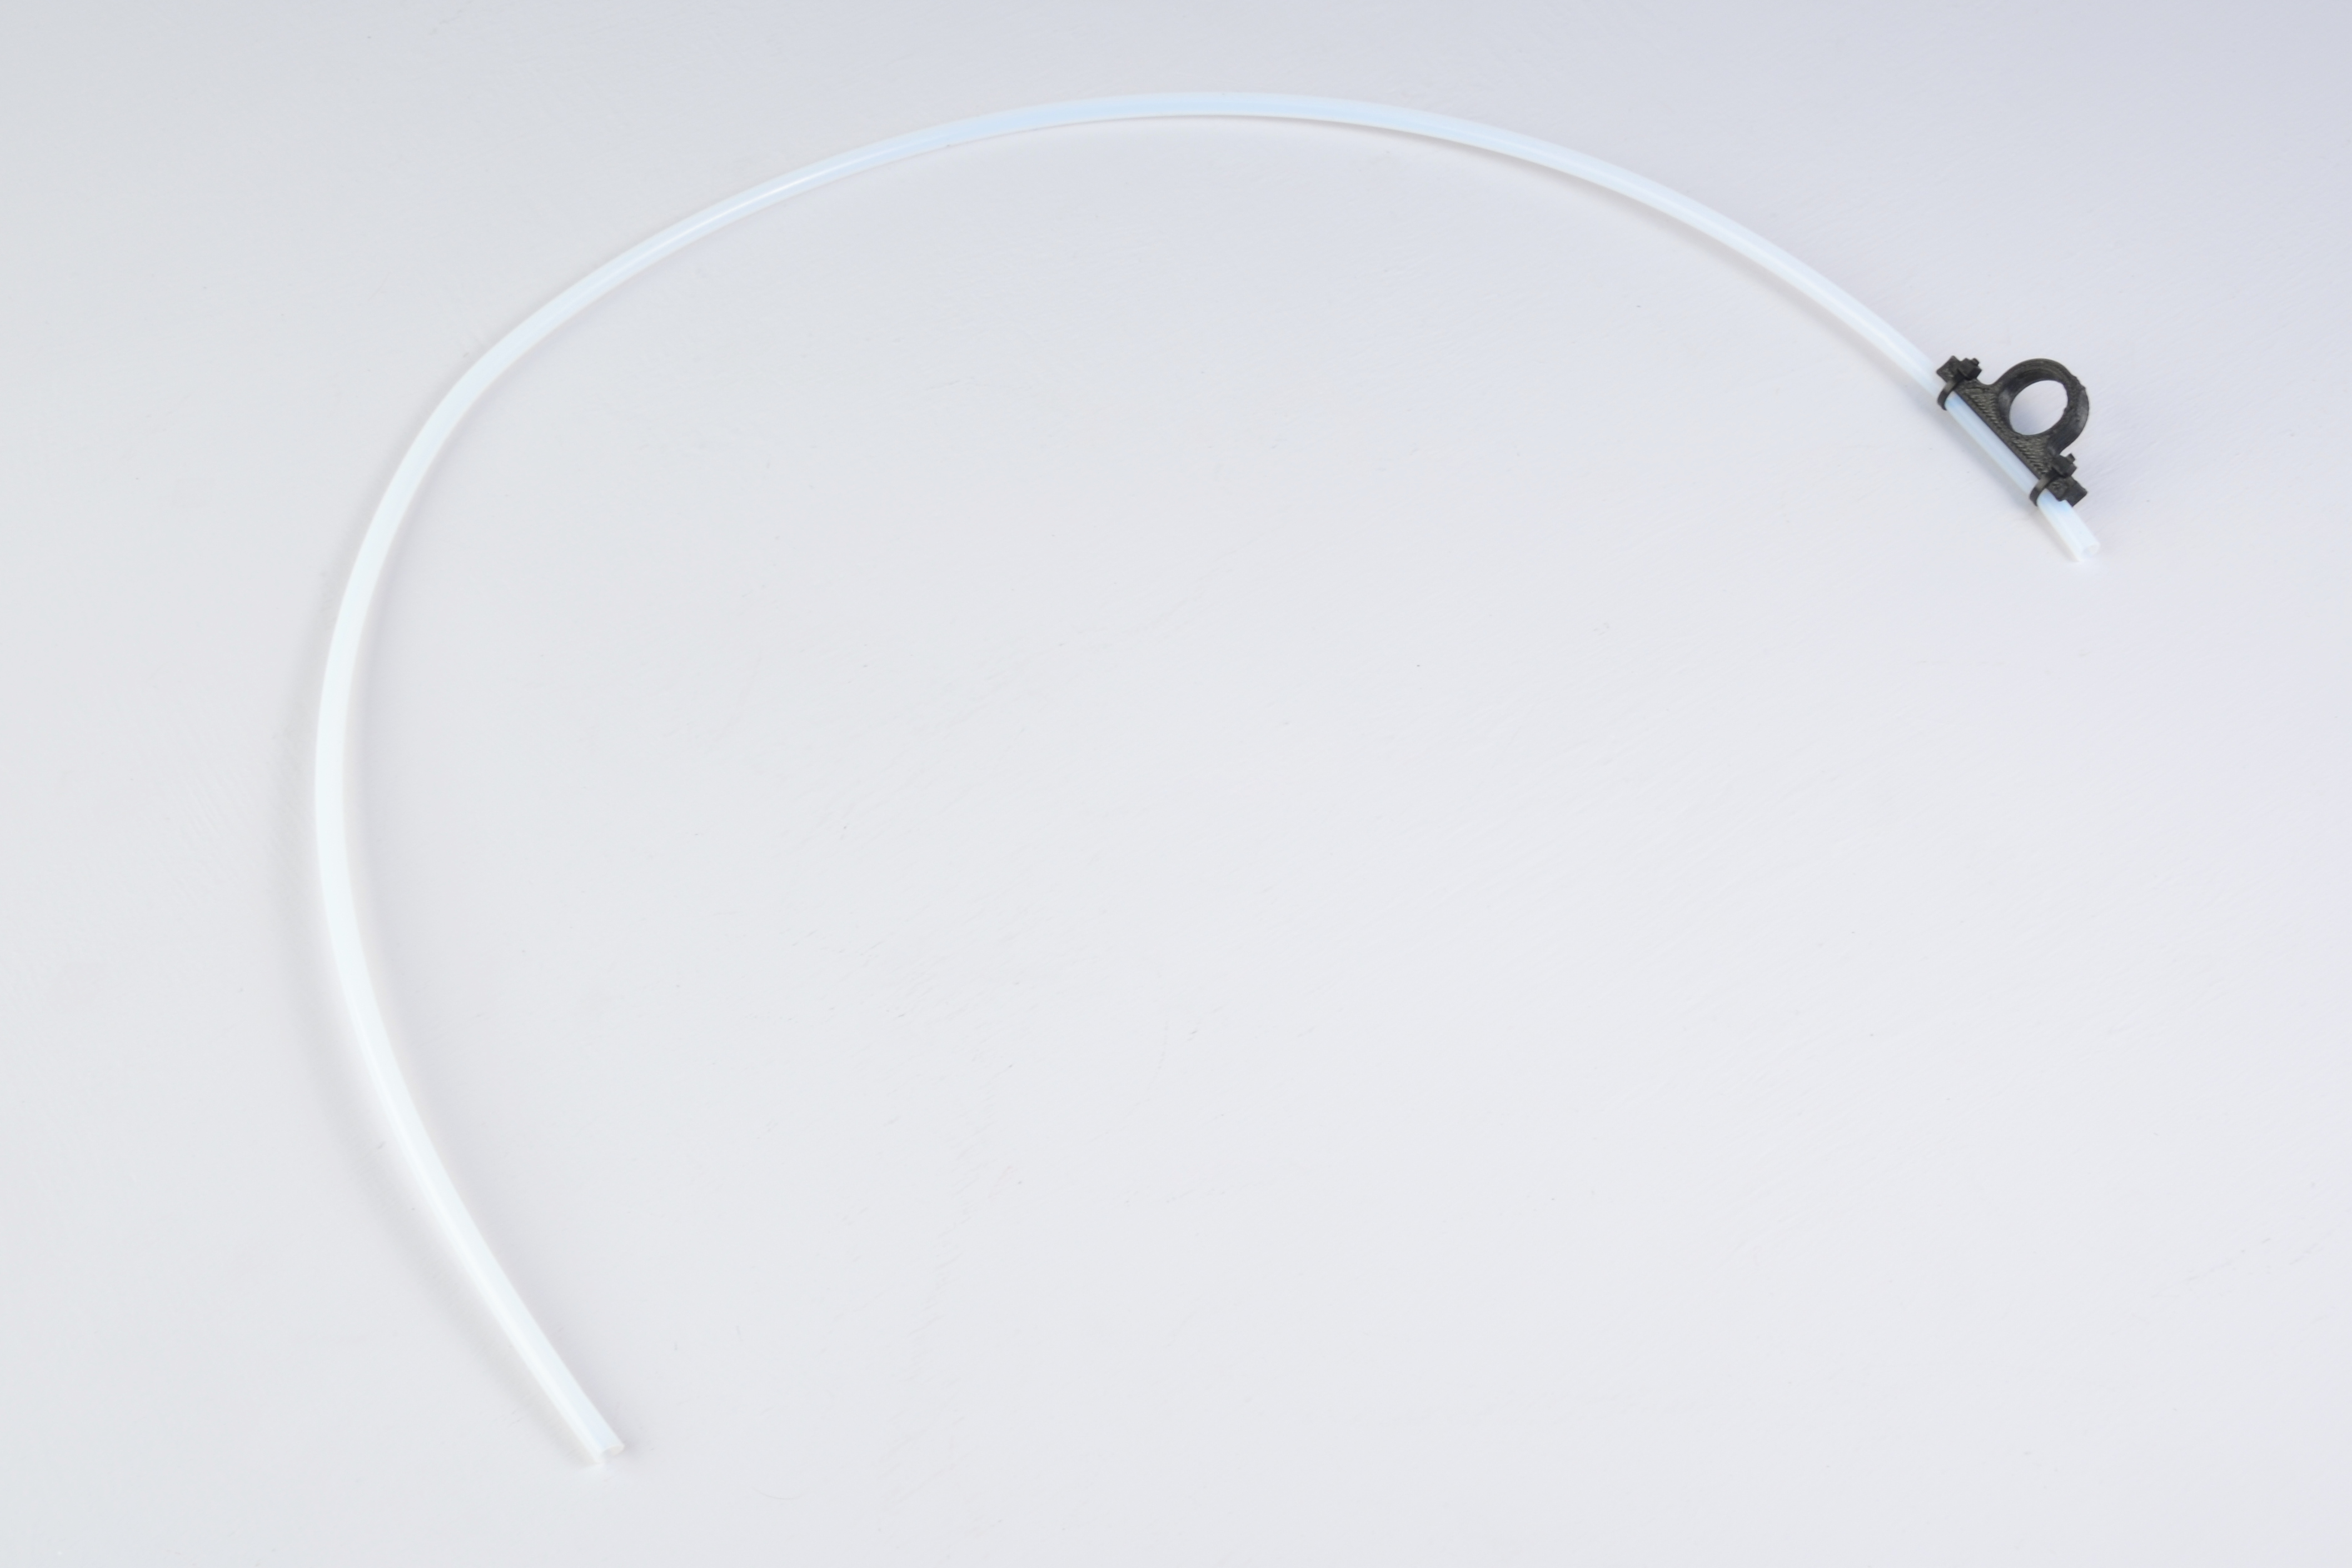
\includegraphics[keepaspectratio=true,angle=0,height=0.4\textheight,width=1.0\textwidth]{filament_guide.JPG}
\caption{Filament Guide}
\label{fig:filament_guide}
\end{figure}

%\begin{figure}[hbt]
\begin{figure}[H]
\centering
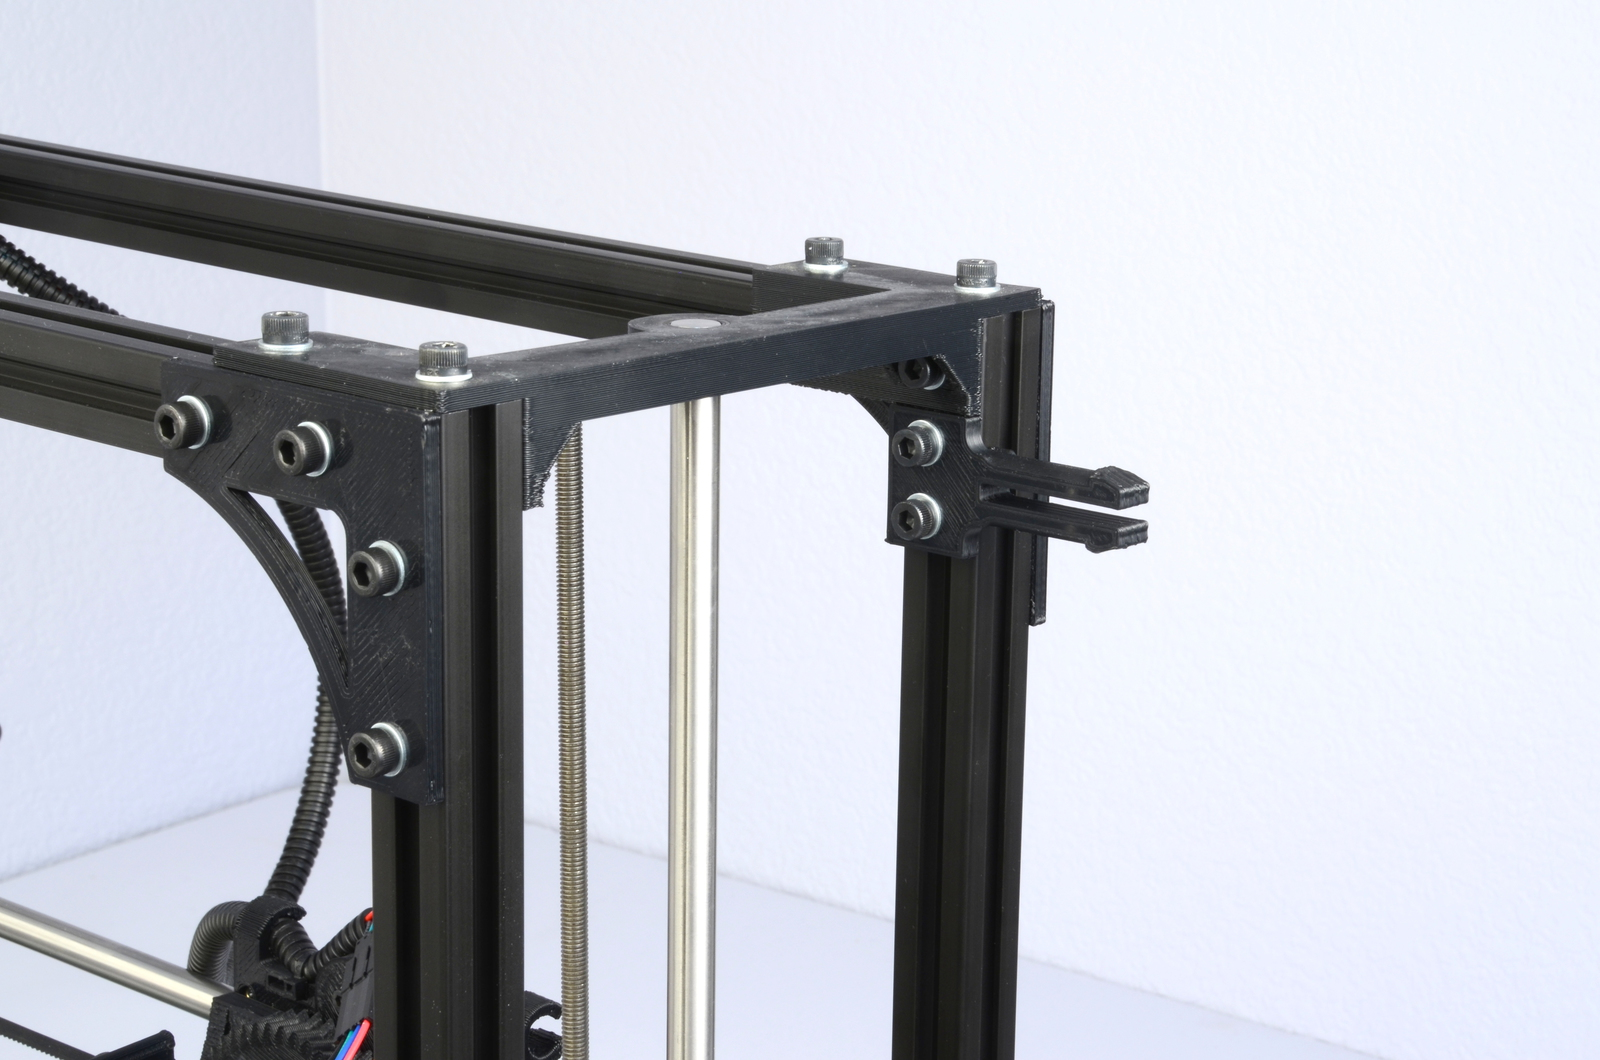
\includegraphics[keepaspectratio=true,angle=0,height=0.4\textheight,width=1.0\textwidth]{filament_guide_mount.JPG}
\caption{Filament Guide Mount}
\label{fig:filament_guide_mount}
\end{figure}

%\begin{figure}[hbt]
\begin{figure}[H]
\centering
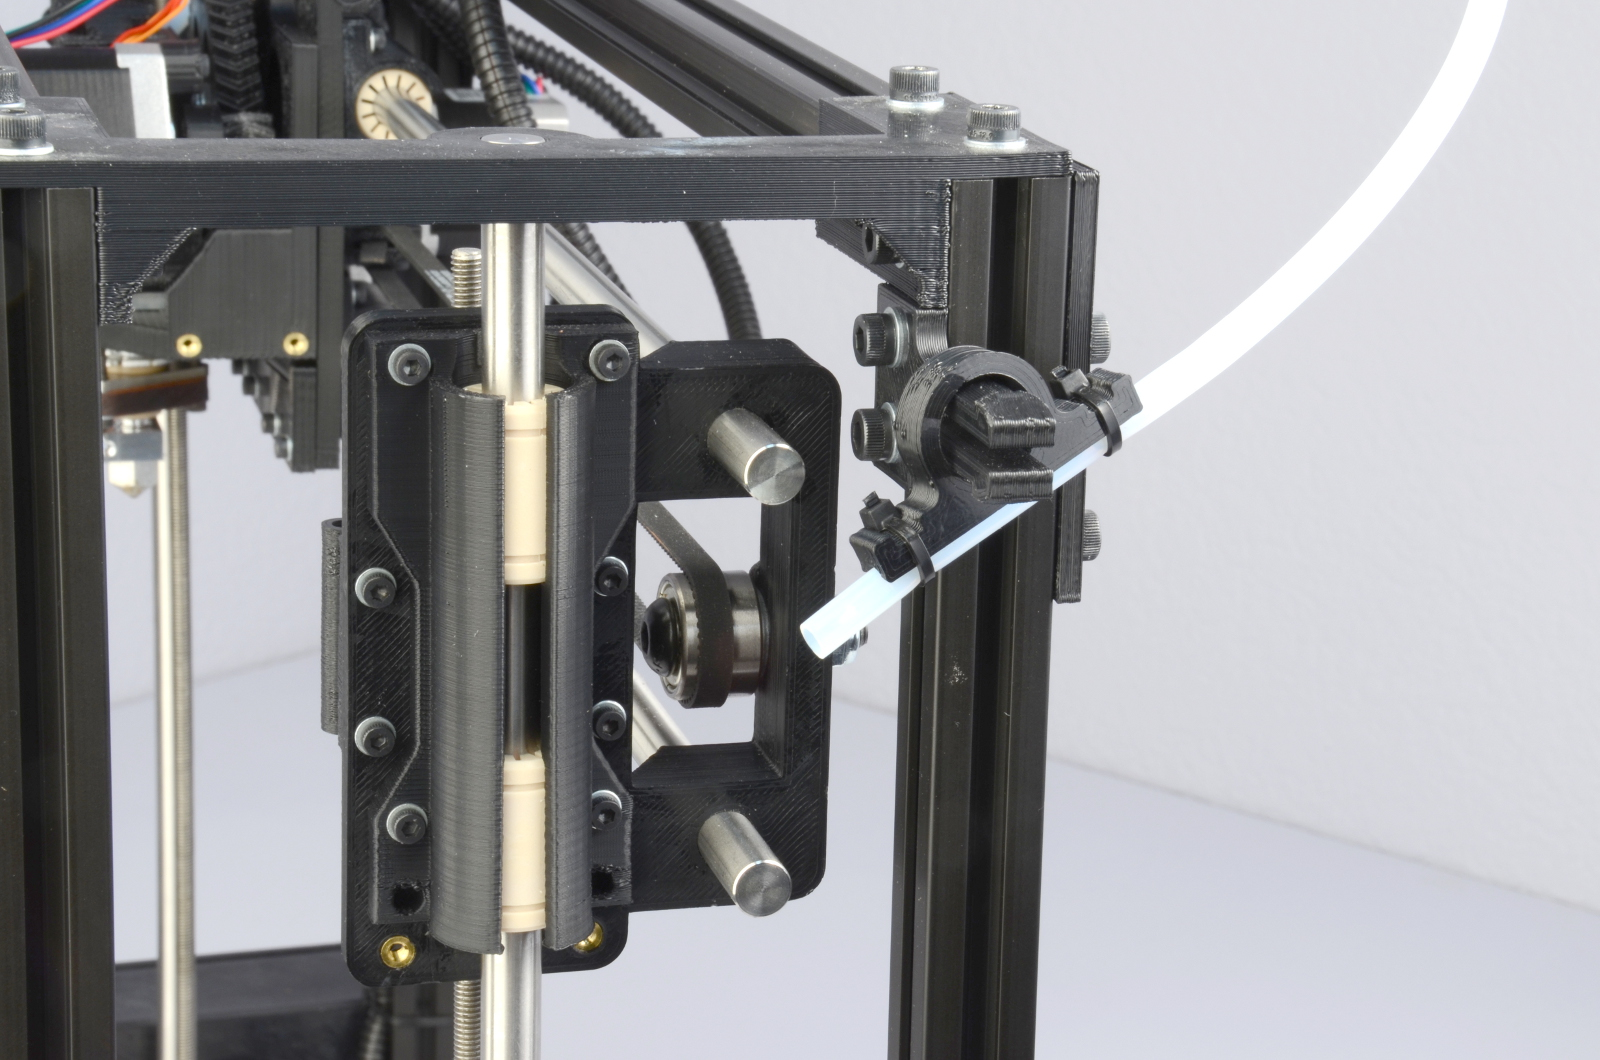
\includegraphics[keepaspectratio=true,angle=0,height=0.4\textheight,width=1.0\textwidth]{filament_guide_direction.JPG}
\caption{Filament Guide Setting}
\label{fig:filament_guide_setting}
\end{figure}

\index{end stops}
\glossary{End stops}{Mechanical or optical switches that are used to mark the 3 home (zero) positions.}
\item Your TAZ 3D printer is now setup and ready to start printing. Before moving forward you should become familiar with the TAZ Cartesian type system. The printer moves in three axes: X, Y, and Z (Fig. \ref{fig:axes}, page \pageref{fig:axes}). These three axes allow the tool head to move to any point within the print area. Note the location of the mechanical end stops which are small switches located at the home point of each axis (Fig. \ref{fig:endstops}, page \pageref{fig:endstops}). Each end stop switch allows the printer to find the 0, the origin, or starting point, of each axis. The mechanical end stops should never be blocked during the initial homing function or during a print.
%\begin{figure}[hbt]
\begin{figure}[H]
\centering
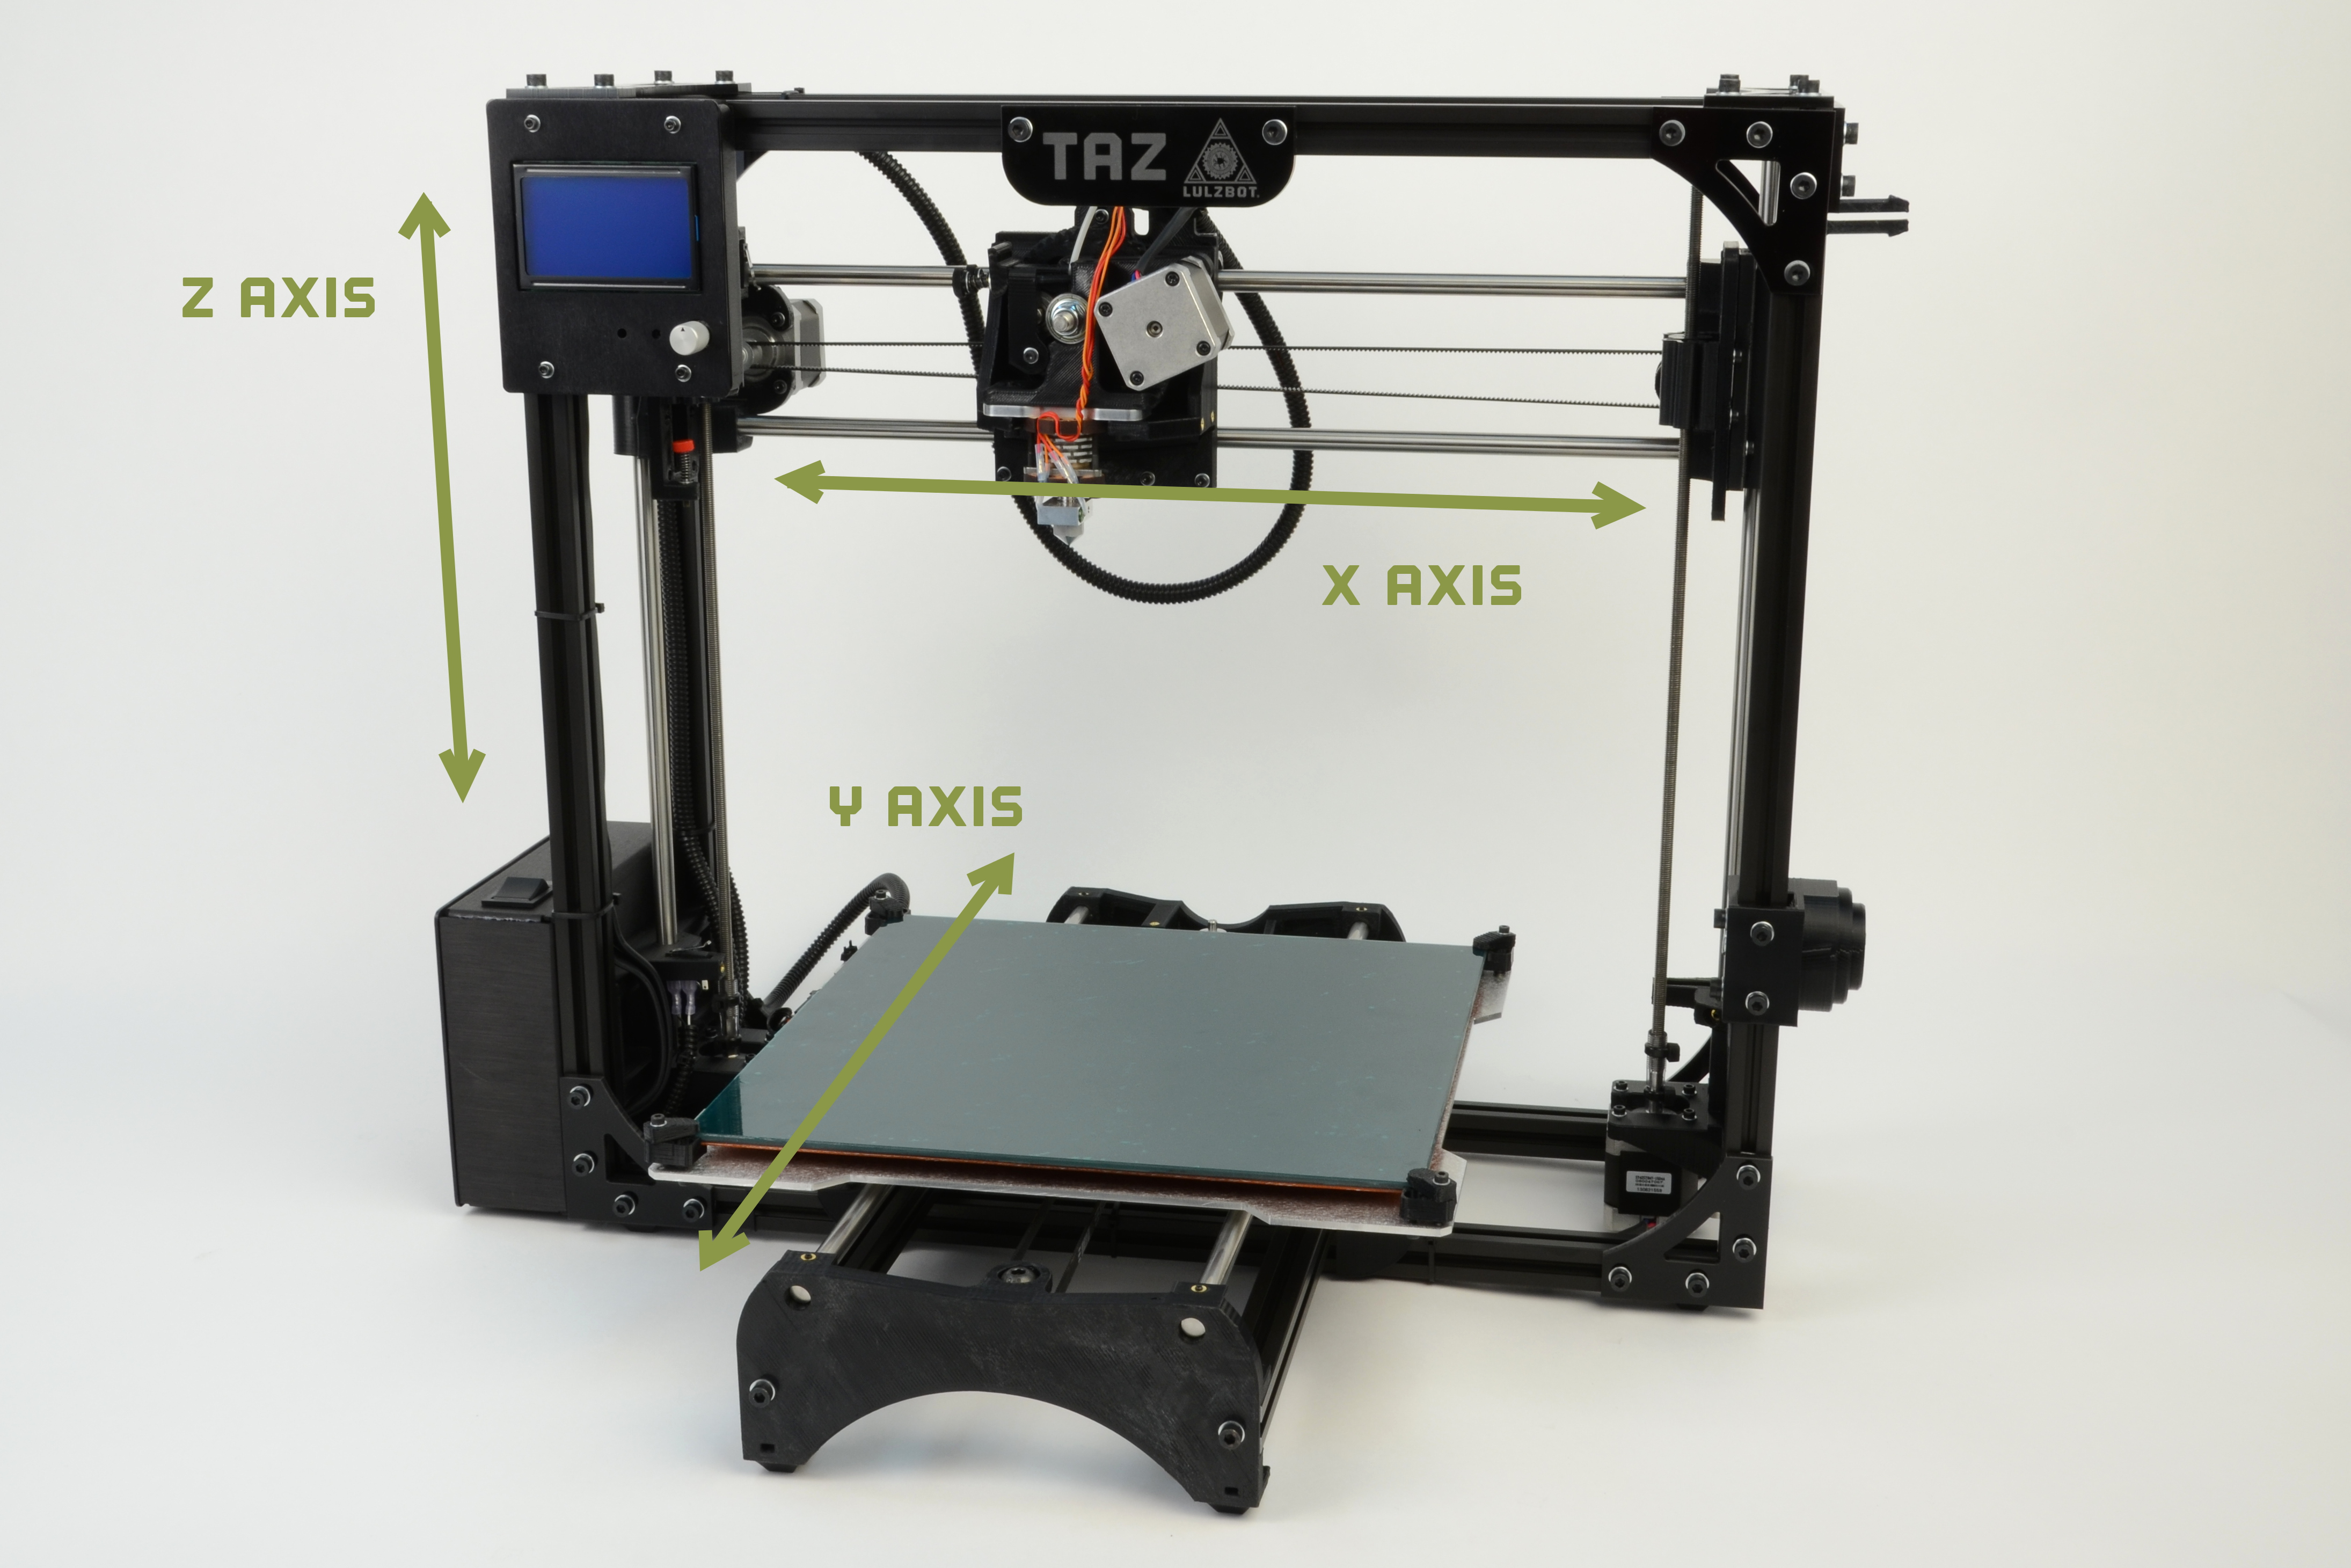
\includegraphics[keepaspectratio=true,angle=0,height=0.4\textheight,width=1.0\textwidth]{axes.JPG}
\caption{Axes movement directions}
\label{fig:axes}
\end{figure}

\begin{figure}[H]
\centering
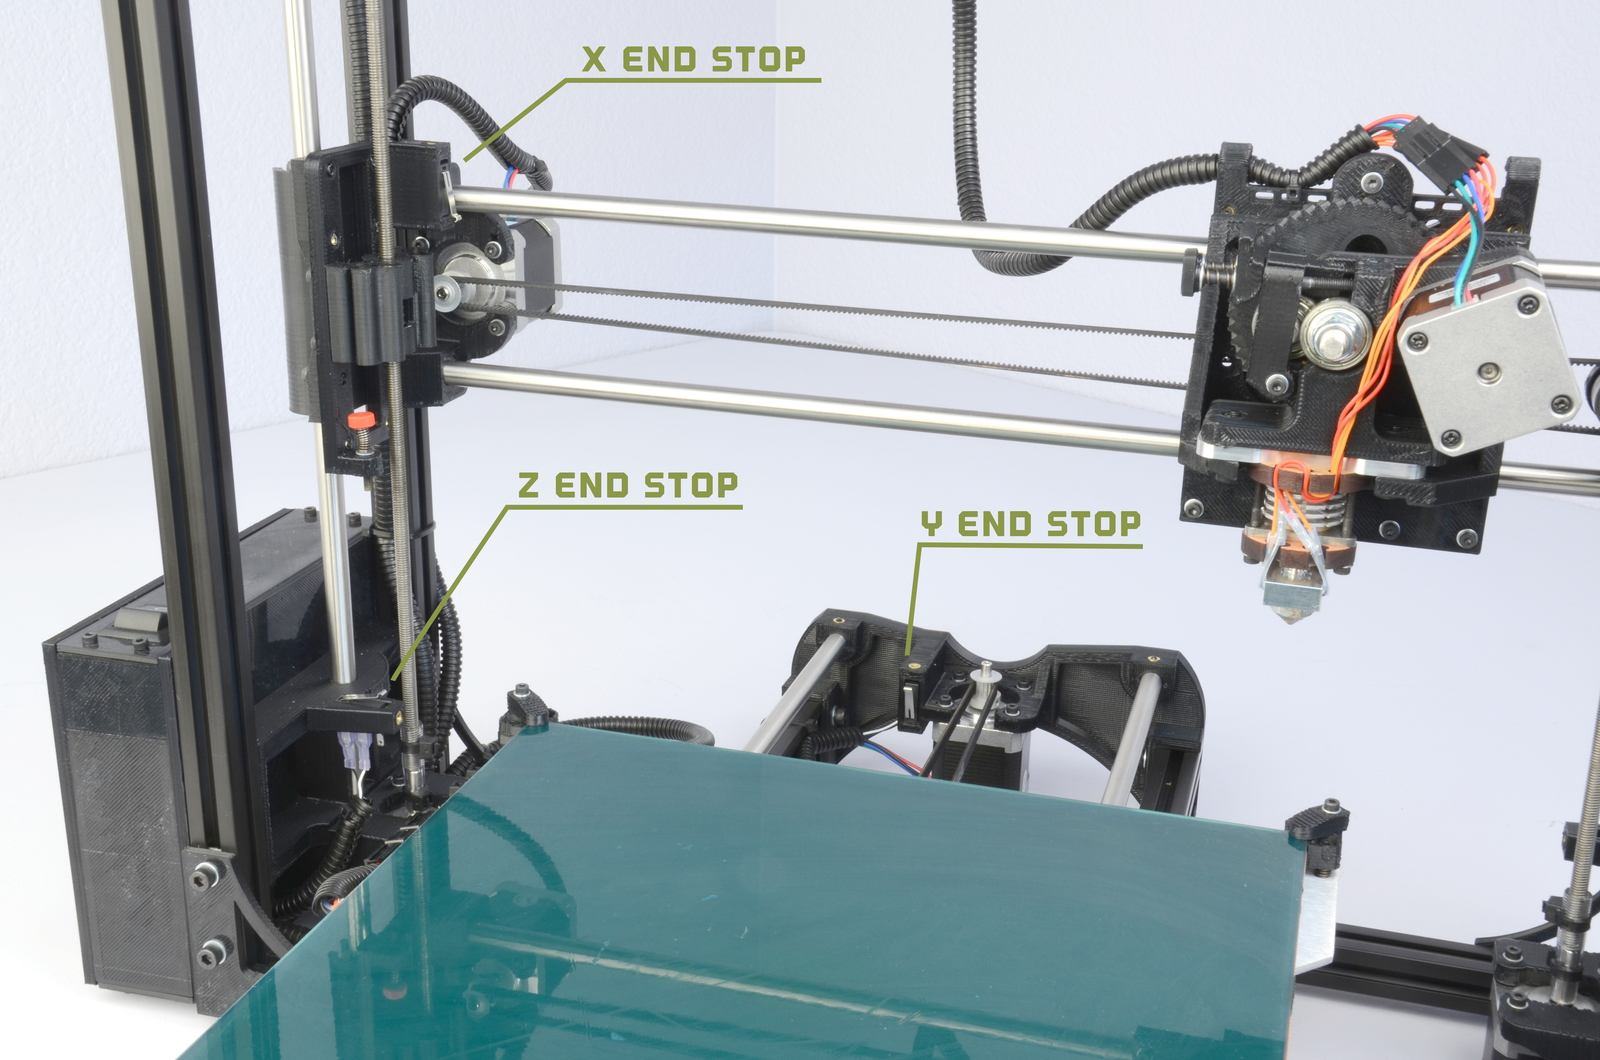
\includegraphics[keepaspectratio=true,angle=0,height=0.4\textheight,width=1.0\textwidth]{end_stop_switches.JPG}
\caption{End stop locations}
\label{fig:endstops}
\end{figure}


\section{ABS \& Acetone Solution Prep}
Please refer to section \ref{sec:ABS/Acetone Glue} (page \pageref{sec:ABS/Acetone Glue}) for instructions in preparing the ABS/Acetone Glue for use when printing with ABS. As it will take some time to dissolve the ABS into the acetone it may now be a good time to make the solution. If you are printing with PLA, the ABS and Acetone solution is not needed.

\begin{comment}
\index{driver}
\section{Installing Drivers}
Linux and Mac OSX users will not need to install a driver to communicate with the TAZ 3D printer. Windows users will. The drivers can be downloaded from \texttt{LulzBot.com/support/downloads}. A visual guide showing the driver installation process can be found in our download section as well.

\index{pronterface}
\index{printrun}
\index{pronsole}
\index{plater}
\index{stl}
\section{Installing Printrun}
Printrun contains several different applications that can be used to control the TAZ 3D printer. It can be installed on Windows, Mac OSX and Linux based computers. Most users will use Pronterface, the graphical user interface for printrun, when using a host software to interact with the 3D printer. \texttt{Pronsole} allows printing from the command line, and can be used for scripting and some automation. \texttt{Plater} allows you to arrange and combine several STL files into one. More information on the other programs within the Printrun package can be found at \texttt{https://github.com/kliment/Printrun}. Printrun can be downloaded from \texttt{LulzBot.com/support/downloads}. Download the version for your operating system and extract. You will need an archive manager to extract the files. If you do not have one installed we recommend using 7-zip, which can be downloaded for free at \texttt{www.1-zip.org}.

\begin{itemize}
\subsection{Windows Instructions}
\index{windows}
\item Once downloaded, extract the \texttt{dist} folder to a location of your choice. You can rename the \texttt{dist} folder if you like. Double click \texttt{pronterface.exe} to run Pronterface.


\subsection{Mac OSX Instructions}
\item Once downloaded, extract the \texttt{dist} folder to a location of your choice. Once extracted, double click the \texttt{pronterface-mac-Mar2012.app} file to install.

\subsection{Linux Instructions}
%\begin{itemize}
\item Once downloaded, extract the \texttt{dist} folder to a location of your choice. You will need to ensure that the following dependencies are met. They are listed in the README.md file. You can use this command to install the dependencies: 
\texttt{sudo apt-get install python-serial python-wxgtk2.8 python-pyglet python-tornado python-setuptools python-libxml2 python-gobject python-pip avahi-daemon libavahi-compat-libdnssd1}
followed by:
\texttt{pip install -r requirements.txt}
Open the \texttt{Printrun-source} folder in a terminal and enter the following command:
\texttt{sudo python setup.py install}.
Run Printrun by issuing the following command:
\texttt{python pronterface.py}
\end{itemize}

\index{printrun}
\section{Using Printrun}

%\begin{figure}[hbt]
\begin{figure}[H]
\centering
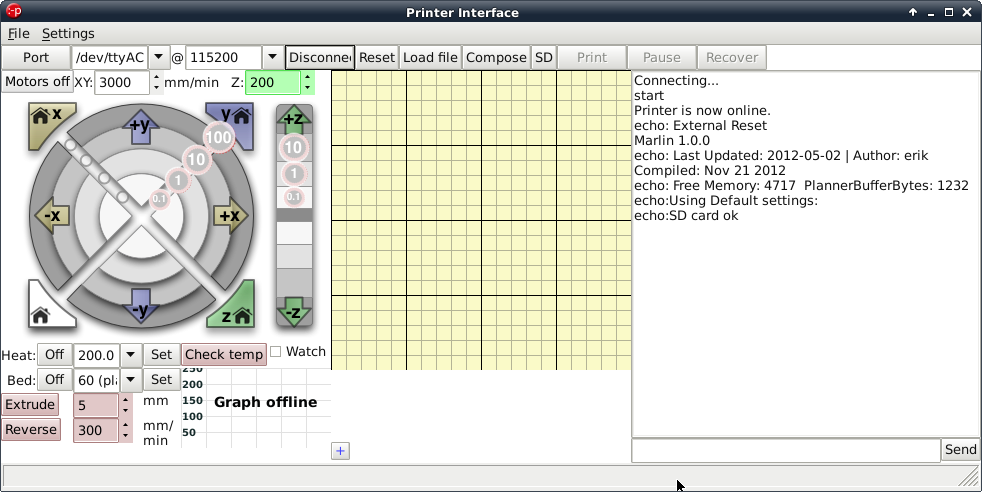
\includegraphics[keepaspectratio=true,angle=0,height=0.4\textheight,width=1.0\textwidth]{printrun.png}
\caption{Printrun}
\label{fig:printrun}
\end{figure}

Printrun is used to control the printer from a computer. It is divided into 4 main parts: The buttons over the top are used to connect to the printer, load files and start \& stop prints.

The movement controls are on the left hand side, with the G-code preview window in the center and the Log window and Terminal command entry box on the right hand side (Fig. \ref{fig:printrun_labels}, page \pageref{fig:printrun_labels}).

\subsection{Connecting to the TAZ 3D Printer}
To connect to the printer, select the correct port by using the drop down arrow and selecting the active port. The \texttt{Port} button will refresh the Port listing. Once selected choose the default \texttt{115200} buad rate and press \texttt{Connect}. Pronterface will open a connection to the printer and display firmware information in the Log window. If nothing is displayed in the Log window verify you have the correct port and connection speed selected. 

%\begin{figure}[hbt]
\begin{figure}[H]
\centering
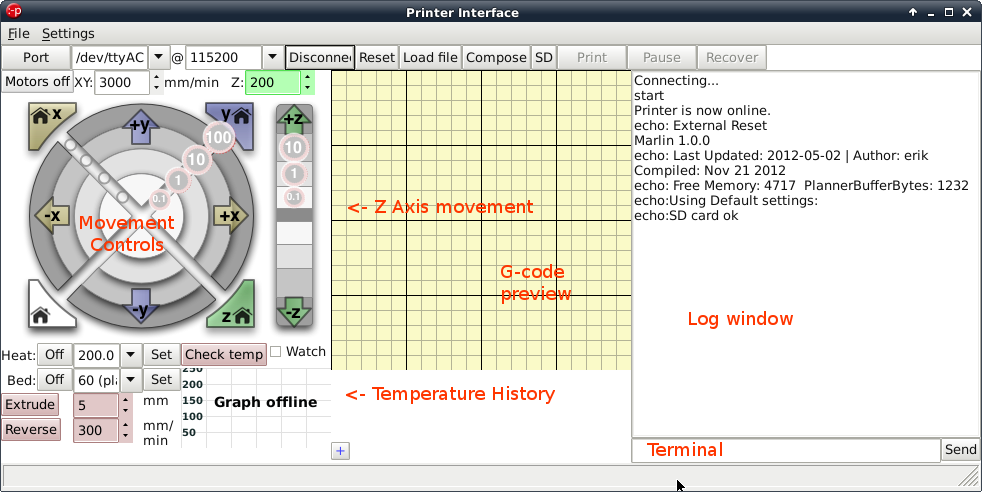
\includegraphics[keepaspectratio=true,angle=0,height=0.4\textheight,width=1.0\textwidth]{printrun-labels.png}
\caption{Printrun Functions}
\label{fig:printrun-labels}
\end{figure}

\subsection{Movement} 
%\begin{figure}[hbt]
\begin{figure}[H]
\centering
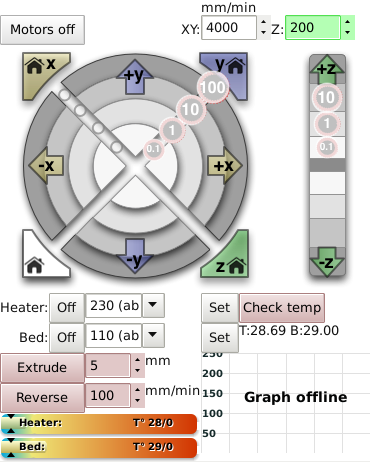
\includegraphics[keepaspectratio=true,angle=0,height=0.4\textheight,width=1.0\textwidth]{printrun_controls.png}
\caption{Movement Controls}
\label{fig:printrun_controls}
\end{figure}

\subsubsection{Motors off}
The TAZ 3D printer can be moved on all three axes independently. If you would like to do so by hand, use the \texttt{Motors off} button to unlock all the stepper motors. Once unlocked they can be moved by hand. Keep in mind that there is no positional feedback, so if you move an axis you will need to re-home in order to re-establish the hot end's position. 

\subsubsection{mm/min ZY:/ Z:}
These settings control the manual jog speeds when driven with Pronterface. Use caution when changing these figures. Moving the axes too fast can cause the printer to lose steps. If that occurs with the Z axis, it can potentially cause the Z axis to become out of square.

\subsubsection{Homing}
Each axes can be homed either individually or together. Press the \texttt{HomeX} button to move the X axis to the left until it activates the end stop. Once the X axis end stop is activated, the X axis carriage will 'bounce'- it will move over and move back to the home position more slowly. Press the \texttt{HomeY} button to home the Y axis. The Y axis platform will move away from you towards the rear of the printer. Press the \texttt{HomeZ} button to home the Z axis. The Z axis will move down towards the heated bed. Make sure that you home the printer immediately after power up. The printer will not know where the not end is until each axes has been homed. Moving prior to home can be risky since the 3D printer will not know it's initial location.  

\subsubsection{X/Y/Z Axes Movement Controls}
Prior to moving the X, Y or Z axis, make sure that you home each axis. The X, Y and Z axes can be moved utilizing the circular movement controls. Each axis can be moved in either fine moves or large moves, ranging from 0.1mm to 100mm.  For example, to move the \texttt{Y Axis} towards you, move your mouse to the \texttt{+y} section until both the \texttt{+y} and the \texttt{100} is highlighted then select that ring section. To move the \texttt{Y axis} away from you, move your mouse to the \texttt{-y} section until both the \texttt{-y} and the \texttt{100} is highlighted then select that ring section. The X axis can be moved in a similar fashion.

The Z axis movement control operates similarly, but the movement scale is different. The Z axis will move in 0.1mm, 1mm and 10mm increments. The top half of the movement bar will move the Z axis up, by the selected units, while the lower half will move the Z axis down, by the desired units. 
\end{comment}

\end{enumerate}
